\documentclass[11pt]{extarticle}
\usepackage[utf8]{inputenc}
\usepackage[T1]{fontenc}
\usepackage[french]{babel}
\usepackage[a4paper]{geometry}
\usepackage[myheadings]{fullpage}
\usepackage{fancyhdr,lastpage,graphicx,setspace,booktabs,array}
\usepackage[font=small,labelfont=bf]{caption}
\usepackage{fourier}
\usepackage[protrusion=true,expansion=true]{microtype}
\usepackage{enumitem,xcolor,listings,float,longtable,placeins}
\captionsetup[table]{position=above}
\setlength{\intextsep}{10pt}
\setlength{\textfloatsep}{10pt}
\setlength{\floatsep}{8pt}
\setcounter{topnumber}{3}
\setcounter{bottomnumber}{2}
\setcounter{totalnumber}{4}
\renewcommand{\topfraction}{0.92}
\renewcommand{\bottomfraction}{0.85}
\renewcommand{\textfraction}{0.08}
\renewcommand{\floatpagefraction}{0.78}
\makeatletter\setlength{\@fptop}{0pt}\setlength{\@fpsep}{10pt}\setlength{\@fpbot}{0pt plus 1fil}\makeatother
\raggedbottom
\setlength{\emergencystretch}{2em}
\pdfimageresolution=72
\usepackage{tikz}
\usetikzlibrary{arrows.meta,positioning,fit,backgrounds,shapes.geometric}
\tikzset{bloc/.style={draw,rounded corners,align=center,text width=3cm,minimum height=1.1cm,fill=blue!5,font=\small},flux/.style={-Latex,thick},note/.style={font=\scriptsize,align=center,text width=1.2cm,fill=white,inner sep=1pt}}
\usepackage[hidelinks]{hyperref}
\onehalfspacing
\setcounter{secnumdepth}{4}
\setcounter{tocdepth}{3}
\newcommand{\HRule}[1]{\rule{\linewidth}{#1}}
\pagestyle{fancy}
\fancyhf{}
\setlength{\headheight}{15pt}
\fancyhead[L]{Yessine Choura}
\fancyhead[R]{IIT SFAX}
\fancyfoot[C]{Page \thepage\ sur \pageref{LastPage}}
\newcommand{\chaptertitle}[2]{\clearpage\phantomsection\begin{center}{\Huge\bfseries #1}\end{center}\vspace{1.5\baselineskip}\addcontentsline{toc}{section}{#1}\setcounter{section}{#2}\setcounter{subsection}{0}}
\newcommand{\fronttitle}[1]{\clearpage\phantomsection\begin{center}{\Huge\bfseries #1}\end{center}\vspace{\baselineskip}\addcontentsline{toc}{section}{#1}}
\lstset{breaklines=true,basicstyle=\ttfamily\small,columns=fullflexible}
% Première version : identité de l'encadrant et intitulé académique à compléter.
% Mise en page inspirée de rapport-pfa.tex ; contenu propre au projet bagages.
\begin{document}\hypersetup{pageanchor=false}
\renewcommand{\contentsname}{\huge\centering\textbf{Table des matières}}
\clearpage{\setstretch{1.12}\tableofcontents}\thispagestyle{empty}
\renewcommand{\listfigurename}{\huge\centering\textbf{Liste des figures}}
\clearpage{\setstretch{1.12}\listoffigures}\thispagestyle{empty}
\renewcommand{\listtablename}{\huge\centering\textbf{Liste des tableaux}}
\clearpage{\setstretch{1.12}\listoftables}\thispagestyle{empty}
\clearpage\pagenumbering{arabic}\hypersetup{pageanchor=true}
\begin{center}{\Huge\bfseries Introduction générale}\end{center}
\phantomsection\addcontentsline{toc}{section}{Introduction générale}
La gestion des bagages associe plusieurs opérations successives, de l’enregistrement à la livraison. La qualité du suivi dépend de la cohérence des changements d’état et de la possibilité d’identifier les interventions des agents. Une modification non autorisée ou une rupture de traçabilité limite la fiabilité des informations communiquées au passager.

Dans ce contexte, le projet étudie la conception d’un système qui associe gestion du parcours et sécurisation de l’infrastructure. La problématique est de fournir un suivi public utile tout en réservant les fonctions internes aux utilisateurs habilités et à un réseau autorisé. La réalisation prend la forme d’un démonstrateur : aucune intégration à un système aéroportuaire réel n’est revendiquée.

L'objectif est de permettre au passager de consulter un suivi limité à l'aide d'un code aléatoire, tout en réservant les opérations internes aux agents authentifiés et connectés au VPN. La protection réseau complète les autorisations applicatives : disposer d'un jeton valide ne suffit pas à atteindre le service privé hors du réseau autorisé.

Le rapport est organisé en trois chapitres. Le premier présente le contexte, la mission, les objectifs, les besoins et l’organisation du travail. Le deuxième traduit ces besoins en une architecture applicative et réseau. Le troisième décrit la réalisation progressive et les validations, avec les captures associées aux étapes correspondantes.
\chaptertitle{Chapitre 1 : Étude préalable et analyse des besoins}{1}
\subsection{Introduction}
L'étude préalable situe la mission et précise le problème auquel la réalisation doit répondre. Elle conduit à définir les objectifs, à examiner les limites d'une gestion sans séparation des accès, puis à proposer une solution cohérente. L'identification des acteurs et des besoins complète cette démarche avant la conception technique.
\subsection{Contexte et définition de la mission}
Le projet s'inscrit dans une démarche de stage orientée vers l'administration des réseaux et la sécurité des infrastructures. La mission consiste à concevoir un démonstrateur de gestion des bagages et à sécuriser son déploiement. Elle associe le développement d'une application fonctionnelle à des vérifications de contrôle d'accès, de segmentation réseau et de persistance.

Le parcours du bagage implique plusieurs responsabilités : enregistrement, manutention, supervision et information du passager. Chaque acteur doit disposer des fonctions nécessaires à son travail sans accéder aux opérations réservées aux autres. L'administrateur gère les comptes au moyen d'une identité dédiée. Aucun organisme d'accueil ni système aéroportuaire réel n'est attribué à cette réalisation ; le périmètre décrit est celui du démonstrateur.
\subsection{Problématique}
La question centrale est la suivante : comment assurer le suivi d'un bagage tout en empêchant les utilisateurs publics d'atteindre les fonctions internes, même s'ils disposent d'un jeton applicatif valide ? Une seconde difficulté concerne la traçabilité : les changements d'état doivent rester compréhensibles, y compris lorsqu'une correction exceptionnelle intervient.

Ces deux dimensions imposent de traiter ensemble les règles métier et la sécurité de l'infrastructure. Un formulaire de connexion ne suffit pas à créer une frontière réseau, tandis qu'un VPN ne décide pas du rôle autorisé à modifier un bagage.
\subsection{Objectifs à atteindre}
La réalisation vise à fournir un suivi public limité au statut et aux horodatages, à enregistrer les bagages associés aux vols et à contrôler leurs transitions. Elle doit conserver les interventions des agents et les motifs des corrections. Sur le plan technique, elle doit limiter les opérations internes au VPN, protéger les échanges par HTTPS et maintenir PostgreSQL dans le réseau privé.

Les livrables attendus comprennent les sources, les configurations Docker et Kubernetes, les scripts de validation, les guides de reproduction et le rapport. Les résultats doivent être observables au moyen de scénarios métier, de contrôles réseau et de captures de l'application réellement exécutée.

\subsection{Critères d'acceptation du démonstrateur}
Une exigence est déclarée validée lorsqu'un scénario identifié produit le résultat attendu et qu'une preuve consigne le contexte d'exécution. Une page affichée ou un conteneur démarré ne suffit donc pas à valider la sécurité. Les critères du tableau~\ref{tab:acceptation} servent de référence à la recette du troisième chapitre.
{\setstretch{1.15}
\begin{longtable}{p{2.8cm}p{6.7cm}p{3.8cm}}
\caption{Critères d'acceptation et preuves attendues}\label{tab:acceptation}\\\toprule
\textbf{Exigence} & \textbf{Condition de réussite} & \textbf{Preuve attendue}\\\midrule\endfirsthead
\toprule\textbf{Exigence} & \textbf{Condition de réussite} & \textbf{Preuve attendue}\\\midrule\endhead
Suivi public & Un code fictif connu retourne le statut et les horodatages sans identité du passager ; les routes privées ne sont pas relayées. & Réponses HTTP et consultation publique.\\
Autorisations & L'action permise aboutit ; une requête sans JWT est refusée et un rôle insuffisant ne modifie pas les données. & Recette métier et contrôles 401/403.\\
Frontière VPN & Avec le même JWT encore valide, l'accès privé fonctionne avec le tunnel, devient inaccessible à sa coupure, puis revient après rétablissement. & Série VPN actif, coupé, rétabli depuis un client identifié.\\
Cycle et historique & Une transition autorisée change le statut et ajoute un événement daté lié à l'agent ; une correction nécessite le rôle et le motif prévus. & Réponses métier et historique consulté.\\
Base privée & Les ports sensibles documentés ne sont pas accessibles depuis les clients extérieurs testés, en IPv4 et IPv6 sur OVH. & Résultats des sondes et configuration des services.\\
Persistance et reprise & Les données contrôlées restent présentes après remplacement du pod et redémarrage ; un dump peut être restauré dans une base distincte. & Comparaison avant/après et compte rendu de restauration.\\\bottomrule
\end{longtable}}
Les critères définissent un périmètre de démonstration. La disponibilité sous forte charge, la perte complète d'un disque et une résistance à toutes les attaques ne sont pas déduites de ces vérifications.

\subsection{Analyse et critique de l'existant}
L'analyse porte ici sur un scénario de référence pédagogique : une application où les opérations internes et le suivi passager seraient accessibles par le même point d'entrée, avec une protection reposant principalement sur la connexion utilisateur. Il ne s'agit pas d'un audit d'un système d'aéroport existant.

Dans ce scénario, le masquage des actions dans l'interface ne garantit pas leur protection face à des appels directs à l'API. Une exposition de la base de données élargit aussi la surface accessible. Enfin, une mise à jour du statut sans conservation de l'agent, de l'heure et du motif rend les anomalies difficiles à expliquer. Ces limites motivent la séparation des services, l'autorisation côté API et l'historique des transitions.
\subsection{Solution proposée}
La solution distingue une application publique de suivi et une application privée destinée aux agents. Le proxy public relaie exclusivement le suivi en lecture. Les fonctions internes nécessitent un chemin réseau WireGuard, une authentification JWT valide et un rôle approprié. PostgreSQL conserve les données métier et l'historique dans un segment privé.

La mise en œuvre commence dans un environnement local reproductible, puis évolue vers Kubernetes et un VPS OVH. Les vérifications accompagnent cette progression : chaque frontière ajoutée doit être testée, et chaque changement de déploiement doit préserver les fonctions déjà réalisées.
\subsection{Méthodologie et organisation du travail}
Le travail suit une démarche incrémentale. Chaque étape possède un objectif, des livrables et une condition de validation. La base et l'API précèdent les interfaces ; les parcours métier précèdent les tests réseau ; le déploiement local précède l'hébergement distant. Les guides consignent les commandes et les limites, tandis que les captures servent de preuves visuelles.

Cette organisation reprend la progression étude, analyse, conception, réalisation et validation du rapport de licence fourni comme modèle. Elle ne suppose pas l'existence d'une équipe Scrum ou de cérémonies qui n'ont pas été documentées pour ce projet.
\subsection{Planning de référence sur six semaines}
Le tableau suivant répartit les activités sur six semaines de stage, sans dates calendaires. Il présente une organisation de référence des tâches ; les preuves techniques conservent leurs dates d'exécution propres et ne sont pas réattribuées artificiellement à ces semaines.
\begin{longtable}{p{1.7cm}p{6.5cm}p{5.2cm}}
\caption{Organisation des activités et livrables sur six semaines}\label{tab:planning-stage}\\
\toprule\textbf{Période} & \textbf{Activités} & \textbf{Livrables et jalon}\\\midrule\endfirsthead
\toprule\textbf{Période} & \textbf{Activités} & \textbf{Livrables et jalon}\\\midrule\endhead
Semaine 1 & Cadrage, analyse des besoins, acteurs, règles métier et conception du modèle de données. & Cahier des charges, modèle relationnel et architecture cible.\\
Semaine 2 & API .NET, migrations PostgreSQL, JWT, rôles, historique et premiers conteneurs. & API reliée à la base ; suivi public et contrôles d'autorisation vérifiés.\\
Semaine 3 & Applications Angular, parcours d'enregistrement et de tri, suivi passager et administration. & Interfaces intégrées ; parcours métier et corrections motivées vérifiés.\\
Semaine 4 & Segmentation Docker, proxys public/privé, TLS, WireGuard et durcissement. & Accès privé avec VPN ; coupure et refus hors VPN contrôlés.\\
Semaine 5 & Kubernetes, stockage persistant, NetworkPolicy et essais depuis Windows et VMware. & Déploiement reproductible ; persistance et protections réseau vérifiées.\\
Semaine 6 & Préparation de l'hébergement, recette finale, sauvegarde/restauration et rédaction. & Dossier de validation, captures légendées et rapport ; hébergement OVH documenté comme prolongement de démonstration.\\\bottomrule
\end{longtable}
Le planning rend visible la dépendance entre les activités plutôt qu'un découpage indépendant de tâches. La documentation et les vérifications accompagnent toutes les semaines. La préparation de l'hébergement est distinguée de sa validation distante effective, détaillée dans le chapitre de réalisation.
\subsection{Présentation du projet}
Le système couvre l'enregistrement, le tri, le chargement, le transport et la livraison des bagages. Les données de démonstration sont fictives. Le projet ne revendique aucune intégration à un système réel d'aéroport ou à un dispositif matériel de lecture.
\subsection{Acteurs et responsabilités}
\begin{table}[htbp]\centering
\caption{Acteurs et responsabilités dans l'application}
\begin{tabular}{p{3.6cm}p{10cm}}\toprule
\textbf{Acteur} & \textbf{Responsabilité}\\\midrule
Passager & Consultation du statut et des horodatages avec un code de suivi.\\
Agent d'enregistrement & Enregistrement et consultation des bagages selon les permissions.\\
Agent de tri & Transitions de manutention autorisées.\\
Superviseur & Gestion des vols et corrections exceptionnelles motivées.\\
Administrateur & Gestion des comptes, sans héritage automatique des droits métier.\\\bottomrule
\end{tabular}\end{table}
\subsection{Besoins fonctionnels}
Le système doit enregistrer les bagages associés aux vols, contrôler les transitions de statut, conserver chaque événement et fournir un suivi public qui ne révèle pas l'identité du passager. Les corrections exceptionnelles nécessitent une autorisation spécifique et un motif.
\subsection{Besoins de sécurité}
Les opérations privées exigent simultanément un accès réseau autorisé, une authentification valide et un rôle compatible avec l'action. La base de données ne doit pas être exposée publiquement. Les mots de passe sont hachés ; les jetons sont limités dans le temps. La sauvegarde et la restauration doivent être vérifiées.
\subsection{Traçabilité et sécurité des données}
La traçabilité repose sur la conservation des changements d'état d'un bagage. Chaque événement permet de comprendre le parcours enregistré et les interventions des agents. Le suivi public est volontairement limité : il expose le statut et les horodatages, sans afficher l'identité du passager. Le code de suivi doit lui-même être conservé de manière confidentielle par son détenteur.
\subsection{Authentification et contrôle d'accès}
L'authentification identifie le compte qui effectue une requête. L'autorisation détermine ensuite si son rôle permet l'opération. Un jeton JWT signé transmet des informations d'identité vérifiées par l'API. Le format JWT~\cite{jwt} est défini par la RFC 7519. Dans ce projet, sa durée de validité est de quinze minutes ; la signature, l'émetteur, le destinataire, l'expiration et l'état du compte sont contrôlés.

Le contrôle par rôle distingue l'enregistrement, le tri, la supervision et l'administration. L'administrateur ne possède pas automatiquement les permissions métier. Le masquage des boutons dans l'interface facilite l'usage, mais l'API reste responsable de la décision d'autorisation.
\subsection{TLS et réseau privé virtuel}
TLS protège les échanges HTTPS entre le client et le service. Le certificat public du VPS est reconnu par les clients testés. L'interface agents utilise une autorité de certification privée installée sur le poste de démonstration.

WireGuard~\cite{wireguard} encapsule les paquets IP dans un tunnel chiffré utilisant UDP. Dans le projet, les pairs configurés accèdent au réseau privé par ce tunnel. Le tunnel ne remplace pas l'authentification applicative : un client connecté doit encore présenter un jeton valide et disposer du rôle approprié. Inversement, un jeton valide n'ouvre pas un chemin réseau vers les fonctions internes en l'absence du tunnel.
\subsection{Conteneurisation et orchestration}
Docker~\cite{docker} exécute les composants dans des conteneurs, c'est-à-dire des processus isolés accompagnés de leurs fichiers nécessaires. Les NetworkPolicies de Kubernetes~\cite{kubernetes} permettent de définir les communications autorisées entre les pods. Kubernetes organise aussi les déploiements, les services et la persistance. La réalisation utilise k3s dans k3d, avec un seul nœud. Les politiques réseau autorisent seulement les flux nécessaires entre les proxys, l'API, la base et le DNS. Cette configuration améliore la séparation des composants sans apporter de haute disponibilité.
\subsection{Conclusion du chapitre}
L'analyse des besoins conduit à distinguer deux axes complémentaires : la gestion fiable du parcours métier et la limitation des accès aux services internes. Le chapitre suivant présente leur traduction dans l'architecture et le modèle de données.
\chaptertitle{Chapitre 2 : Conception de l’architecture proposée}{2}
\subsection{Cas d'utilisation et responsabilités}
Le diagramme de la figure~\ref{fig:cas-utilisation} associe chaque acteur à son groupe de fonctions. Les opérations internes exigent le VPN et une session autorisée. Le superviseur peut enregistrer des bagages et effectuer des transitions ; sa responsabilité particulière porte sur les vols et les corrections motivées. L'administrateur reste séparé des opérations métier.
\begin{figure}[H]\centering
\resizebox{0.95\linewidth}{!}{%
\begin{tikzpicture}[cas/.style={ellipse,draw,align=center,text width=6cm,minimum height=1.15cm,fill=blue!5,font=\small},acteur/.style={align=center,text width=3.6cm,font=\small}]
\node[acteur] (p) at (0,0) {Passager};
\node[acteur] (e) at (0,-1.8) {Agent d'enregistrement};
\node[acteur] (t) at (0,-3.6) {Agent de tri};
\node[acteur] (s) at (0,-5.4) {Superviseur};
\node[acteur] (a) at (0,-7.2) {Administrateur};
\node[cas] (cp) at (7,0) {Consulter le suivi par code\\Lecture publique};
\node[cas] (ce) at (7,-1.8) {Enregistrer un bagage\\Associer le vol et produire le reçu};
\node[cas] (ct) at (7,-3.6) {Consulter les bagages et l'historique\\Effectuer les transitions autorisées};
\node[cas] (cs) at (7,-5.4) {Gérer les vols et superviser\\Corriger une anomalie avec motif};
\node[cas] (ca) at (7,-7.2) {Gérer les comptes utilisateurs};
\foreach \x/\y in {p/cp,e/ce,t/ct,s/cs,a/ca}{\draw (\x.east)--(\y.west);}
\begin{scope}[on background layer]
\node[draw,fit=(ce)(ct)(cs)(ca),inner sep=.3cm,label={[font=\small]right:VPN + JWT + rôle}] {};
\end{scope}
\end{tikzpicture}}
\caption{Cas d'utilisation regroupés par responsabilité et périmètre d'accès}
\label{fig:cas-utilisation}
\end{figure}
\subsection{Architecture générale}
Angular~\cite{angular} fournit le cadre de développement des interfaces web. Dans notre architecture, deux applications Angular sont servies par des proxys Nginx distincts. Le proxy public autorise uniquement le suivi en lecture. Le proxy agents est accessible par WireGuard et transmet les opérations privées à l'API. PostgreSQL reste dans le réseau interne.

\begin{figure}[H]\centering
\resizebox{0.98\linewidth}{!}{%
\begin{tikzpicture}
\node[bloc] (passager) at (0,2.2) {Passager\\Code de suivi};
\node[bloc] (public) at (4.3,2.2) {Angular 22 public\\Nginx : suivi seul};
\node[bloc] (agent) at (0,-1.2) {Agents et superviseur\\Administrateur dédié};
\node[bloc] (prive) at (4.3,-1.2) {Angular 22 agents\\Nginx privé};
\node[bloc,fill=green!8] (api) at (8.6,0.5) {API ASP.NET Core\\JWT et rôles};
\node[bloc,fill=orange!10] (db) at (12.9,0.5) {PostgreSQL 16\\Données et historique};
\draw[flux] (passager)--node[above=3mm,note]{HTTPS} (public);
\draw[flux] (agent)--node[above=3mm,note]{VPN puis HTTPS} (prive);
\draw[flux] (public.east)-|node[pos=.3,above,note]{Lecture du suivi} (api.north);
\draw[flux] (prive.east)-|node[pos=.3,below,note]{Actions\\privées} (api.south);
\draw[flux] (api)--node[above=3mm,note]{Accès SQL privé} (db);
\end{tikzpicture}}
\caption{Architecture applicative proposée et réalisée : séparation des interfaces et contrôle des opérations}
\label{fig:architecture-applicative}
\end{figure}
La figure~\ref{fig:architecture-applicative} présente les responsabilités des composants. Le site passager utilise uniquement le suivi public, tandis que les agents accèdent aux opérations internes. Les deux chemins aboutissent à l'API, qui applique les règles métier avant toute interaction avec PostgreSQL. Angular fournit les interfaces utilisateur et PostgreSQL assure la persistance relationnelle.
\subsection{Architecture réseau de l'hébergement OVH}
\begin{figure}[H]\centering
\resizebox{0.95\linewidth}{!}{%
\begin{tikzpicture}
\node[bloc] (pubclient) at (0,2.5) {Passager sur Internet};
\node[bloc] (vpnclient) at (0,-1) {Client autorisé\\Windows ou VM};
\node[bloc] (tls) at (4.6,2.5) {VPS OVH : TCP 443\\HTTPS public};
\node[bloc,fill=green!8] (wg) at (4.6,-1) {VPS OVH : UDP 52820\\WireGuard};
\node[bloc] (priv) at (9.2,-1) {10.77.0.1:8443\\HTTPS agents privé};
\node[bloc,fill=orange!10] (internal) at (9.2,2.5) {Services internes\\API et PostgreSQL};
\draw[flux] (pubclient)--node[above=3mm,note]{Internet} (tls);
\draw[flux] (vpnclient)--node[above=3mm,note]{Tunnel chiffré} (wg);
\draw[flux] (wg)--node[above=3mm,note]{Réseau VPN} (priv);
\draw[flux] (tls)--node[above=3mm,note]{Suivi seulement} (internal);
\draw[flux] (priv)--node[right,note]{JWT et rôle} (internal);
\node[note,draw,dashed,text width=9cm] at (6.8,-3) {Aucun accès public direct à PostgreSQL ni à l'interface agents.\\Le VPN et les autorisations applicatives se complètent.};
\end{tikzpicture}}
\caption{Architecture réseau OVH : accès public HTTPS et accès privé par WireGuard}
\label{fig:architecture-reseau}
\end{figure}
La figure~\ref{fig:architecture-reseau} distingue les connexions publiques et le tunnel privé. WireGuard transporte les paquets réseau chiffrés au-dessus d'UDP. Le port 8443 appartient à l'adresse du VPN : il n'est pas publié comme service privé directement accessible depuis Internet. L'administration SSH par clé constitue un accès de maintenance distinct.
\subsection{Architecture Kubernetes et stockage}
\begin{figure}[H]\centering
\resizebox{0.95\linewidth}{!}{%
\begin{tikzpicture}
\node[bloc] (public) at (0,3) {Deployment public\\Nginx et Angular};
\node[bloc] (wg) at (4.4,3) {Pod passerelle\\WireGuard};
\node[bloc] (agents) at (8.8,3) {Deployment agents\\Service ClusterIP};
\node[bloc,fill=green!8] (api) at (4.4,0) {Deployment API\\Service ClusterIP};
\node[bloc,fill=orange!10] (db) at (8.8,0) {StatefulSet PostgreSQL\\Service ClusterIP};
\node[bloc,fill=orange!10] (pvc) at (8.8,-2.3) {PVC local-path\\Stockage persistant};
\node[bloc] (config) at (0,0) {Secrets et ConfigMaps\\Configuration};
\draw[flux] (public.south)--(0,1.4)--node[above=3mm,note]{Suivi}(4.4,1.4)--(api.north);
\draw[flux] (wg)--node[above=3mm,note]{HTTPS privé} (agents);
\draw[flux] (agents.south)--(8.8,1.1)--(5.7,1.1)--(5.7,0.8)--(api.north);
\draw[flux] (api)-- (db);
\draw[flux] (db)-- (pvc);
\draw[flux,dashed] (config)-- (api);
\begin{scope}[on background layer]
\node[draw,dashed,rounded corners,fit=(public)(wg)(agents)(api)(db)(pvc)(config),inner sep=0.6cm,label={[font=\small]above:VPS OVH -- Docker / k3d -- k3s mono-nœud}] {};
\end{scope}
\end{tikzpicture}}
\caption{Organisation Kubernetes : services privés, configuration et persistance sur un seul nœud}
\label{fig:architecture-kubernetes}
\end{figure}
La figure~\ref{fig:architecture-kubernetes} montre le déploiement de démonstration. Les NetworkPolicies restreignent les flux aux communications explicitement autorisées. Les migrations et l'initialisation sont réalisées par des Jobs. Le volume conserve les données après remplacement du pod PostgreSQL, mais son stockage local ne garantit pas la reprise après perte du nœud.
\subsection{Modèle de données}
PostgreSQL~\cite{postgresql} est le système de gestion de base de données relationnelle utilisé pour cette réalisation. Les tables principales sont \texttt{roles}, \texttt{users}, \texttt{vols}, \texttt{bagages} et \texttt{historique\_statuts}. Un bagage appartient à un vol. Les événements d'historique conservent l'état, la date et l'agent responsable. Le statut et son événement sont enregistrés atomiquement ; le contrôle de concurrence évite les écrasements silencieux.
\begin{figure}[H]\centering
\resizebox{0.95\linewidth}{!}{%
\begin{tikzpicture}[entite/.style={draw,rounded corners,align=left,text width=4cm,fill=blue!5,font=\small,inner sep=8pt},lien/.style={thick},card/.style={font=\small,fill=white}]
\node[entite] (roles) at (0,4) {\textbf{roles}\\\hrulefill\\PK : Name};
\node[entite] (users) at (6,4) {\textbf{users}\\\hrulefill\\PK : Id\\FK : Role $\rightarrow$ roles.Name\\Login, PasswordHash};
\node[entite] (history) at (6,0) {\textbf{historique\_statuts}\\\hrulefill\\PK : Id\\FK : BagageId, AgentId\\Horodatage\\AncienStatut, NouveauStatut};
\node[entite] (vols) at (0,-4) {\textbf{vols}\\\hrulefill\\PK : Id\\Numero, DepartPrevu};
\node[entite] (bags) at (6,-4) {\textbf{bagages}\\\hrulefill\\PK : Id\\FK : VolId\\TrackingId, PoidsKg, Statut};
\draw[lien] (roles)--node[card,pos=.15]{1}node[card,pos=.85]{0..*}(users);
\draw[lien] (users)--node[card,pos=.15]{1}node[card,pos=.85]{0..*}(history);
\draw[lien] (vols)--node[card,pos=.15]{1}node[card,pos=.85]{0..*}(bags);
\draw[lien] (bags)--node[card,pos=.15]{1}node[card,pos=.85]{0..*}(history);
\end{tikzpicture}}
\caption{Modèle relationnel simplifié et cardinalités issues des relations de l'application}
\label{fig:modele-relationnel}
\end{figure}
Le schéma présente les clés et les liens nécessaires à la compréhension du parcours, sans détailler toutes les colonnes. Un compte possède un rôle ; chaque bagage appartient à un vol et chaque événement référence un bagage et un agent. Les relations restrictives évitent de supprimer une entité encore référencée. L'unicité du code de suivi distingue chaque bagage.
\subsection{Cycle de vie d'un bagage}
Le parcours normal est : enregistré, trié, chargé, en vol, livré. Une déclaration de perte interrompt ce parcours. La récupération d'un bagage perdu relève d'une correction motivée du superviseur.
\subsection{Séparation des protections}
Le VPN contrôle l'accès réseau ; JWT identifie le compte ; les rôles autorisent les opérations. Les NetworkPolicies appliquent un refus par défaut puis autorisent les flux nécessaires. Le compte PostgreSQL applicatif peut lire et ajouter l'historique, sans le modifier ni le supprimer. Le propriétaire de la base reste un acteur de confiance.

\subsection{Organisation du code et des responsabilités}
Le backend regroupe les contrats HTTP, les règles métier, l'accès aux données et les contrôles de sécurité. Entity Framework Core décrit les relations et exécute les migrations PostgreSQL. Les applications Angular publique et agents sont compilées séparément afin que le service passager n'embarque pas les écrans internes. Les scripts de démarrage et de validation organisent les expériences ; les manifests déclarent les ressources Kubernetes.
\subsection{Contrat de l'API}
\begin{longtable}{p{5.5cm}p{8cm}}
\caption{Principaux points d'entrée et protections}\\\toprule
\textbf{Route} & \textbf{Usage et contrôle}\\\midrule\endfirsthead
\toprule\textbf{Route} & \textbf{Usage et contrôle}\\\midrule\endhead
\texttt{GET /api/track/\{code\}} & Lecture publique du statut et des événements, sans identité du passager.\\
\texttt{POST /api/auth/login} & Connexion privée, limitation du débit et verrouillage après échecs.\\
\texttt{GET /api/vols} & Consultation autorisée dans le réseau privé.\\
\texttt{POST /api/vols} & Création réservée au superviseur.\\
\texttt{POST /api/bagages} & Enregistrement par un rôle habilité.\\
\texttt{GET /api/bagages} & Liste et filtres selon les permissions.\\
{\footnotesize\texttt{PATCH /api/bagages/\{id\}/statut}} & Transition normale ou correction motivée, contrôlée par l'API.\\
{\scriptsize\texttt{GET /api/bagages/\{id\}/historique}} & Consultation privée de la traçabilité.\\\bottomrule
\end{longtable}
Les réponses distinguent notamment l'absence d'authentification (401), un rôle insuffisant (403), une ressource absente (404), un conflit métier ou concurrent (409) et un débit dépassé (429). Le suivi public ne relaie pas les fonctions de connexion, comptes, vols ou modification des bagages.
\subsection{Description du modèle relationnel}
\begin{table}[H]\centering\caption{Entités et liens du modèle métier}
\begin{tabular}{p{4cm}p{9.5cm}}\toprule
\textbf{Entité} & \textbf{Rôle dans le modèle}\\\midrule
\texttt{roles} & Définit les permissions attribuées aux comptes.\\
\texttt{users} & Compte, mot de passe haché et rôle associé.\\
\texttt{vols} & Référence du vol auquel les bagages sont rattachés.\\
\texttt{bagages} & Données d'enregistrement, vol, statut courant et code de suivi aléatoire.\\
\texttt{historique\_statuts} & Événements datés liés au bagage et à l'agent responsable.\\\bottomrule
\end{tabular}\end{table}
La séparation du statut courant et des événements permet une consultation rapide tout en conservant le parcours. Le contrôle de concurrence utilise \texttt{xmin} PostgreSQL. Une modification concurrente ne doit pas effacer silencieusement une autre transition. Les droits SQL de l'historique limitent le compte applicatif à la lecture et à l'ajout.

\subsection{Justification des choix et compromis}
Les choix sont appréciés au regard de trois contraintes : réaliser un parcours métier complet, rendre les protections vérifiables et conserver un environnement reproductible sur le poste de travail puis sur un VPS. Aucune comparaison de performances entre produits n'a été menée ; le tableau~\ref{tab:choix} présente les raisons de conception, plutôt qu'un classement des technologies.
{\setstretch{1.15}
\begin{longtable}{p{2.5cm}p{3.3cm}p{4.9cm}p{2.7cm}}
\caption{Choix techniques, alternatives et compromis}\label{tab:choix}\\\toprule
\textbf{Choix} & \textbf{Alternative possible} & \textbf{Raison dans ce projet} & \textbf{Compromis}\\\midrule\endfirsthead
\toprule\textbf{Choix} & \textbf{Alternative possible} & \textbf{Raison dans ce projet} & \textbf{Compromis}\\\midrule\endhead
WireGuard & API privée publiée avec authentification seule ; autre VPN. & Ajouter une frontière réseau indépendante du JWT et vérifier sa coupure depuis Windows et Ubuntu. & Configuration et distribution des clés des pairs.\\
PostgreSQL & Autre base relationnelle ; base documentaire. & Les liens bagage--vol--agent et l'historique justifient un modèle relationnel ; les contraintes et transactions soutiennent la cohérence métier. & Migrations et administration de la base nécessaires.\\
Docker puis Kubernetes & Exécution native ; maintien sous Compose. & Compose stabilise d'abord l'exécution ; Kubernetes permet ensuite d'étudier services privés, politiques réseau et stockage persistant. & Complexité supérieure à Compose pour un petit démonstrateur.\\
Deux interfaces Angular & Une interface unique avec menus conditionnels. & Distinguer les usages public et agents ainsi que leurs points d'entrée ; garder les décisions d'autorisation dans l'API. & Deux compilations et deux configurations à maintenir.\\
VPS OVH & Démonstration locale ou dans une VM. & Disposer d'un point d'entrée public pour l'hébergement HTTPS et les validations du VPN depuis Internet. & Abonnement actif et administration de l'hôte.\\\bottomrule
\end{longtable}}
Kubernetes n'est pas indispensable au seul suivi d'un bagage. Son intérêt ici est pédagogique et architectural : appliquer la segmentation et vérifier la persistance dans un environnement orchestré. Le choix d'un seul nœud reste proportionné à la démonstration, mais ne fournit pas de haute disponibilité. De même, séparer deux interfaces facilite le déploiement ; la sécurité dépend toujours des proxys, du VPN et des autorisations côté serveur.
\subsection{Menaces étudiées et protections associées}
Les biens à protéger sont les données des bagages, l'historique, les comptes et les secrets d'accès. Les points d'entrée considérés sont le site public, le service VPN et les routes privées de l'API. L'analyse porte sur un utilisateur extérieur, un utilisateur possédant un JWT et un agent dont le rôle ne permet pas l'action demandée. L'administrateur de l'hôte demeure dans le périmètre de confiance.
{\setstretch{1.15}
\begin{longtable}{p{3.1cm}p{4.6cm}p{3.1cm}p{2.6cm}}
\caption{Lien entre menaces, protections et validations}\label{tab:menaces}\\\toprule
\textbf{Menace} & \textbf{Protection retenue} & \textbf{Vérification} & \textbf{Risque résiduel}\\\midrule\endfirsthead
\toprule\textbf{Menace} & \textbf{Protection retenue} & \textbf{Vérification} & \textbf{Risque résiduel}\\\midrule\endhead
Accès privé depuis Internet & Proxy public limité au suivi ; services privés ; VPN obligatoire. & Routes privées refusées et coupure du tunnel avec le même JWT. & Une mauvaise configuration future peut élargir l'exposition.\\
Réutilisation d'un JWT obtenu par un tiers & Signature, durée limitée, contrôles de compte et rôle ; accès réseau privé distinct. & JWT seul insuffisant hors VPN ; contrôles d'authentification. & JWT et accès VPN compromis ensemble ; poste client compromis.\\
Modification par un rôle non habilité & Autorisation dans l'API et compte administrateur distinct des rôles métier. & Actions permises et interdites dans la recette. & Compromission d'un compte effectivement habilité.\\
Fuite de données par le suivi & Réponse publique limitée et code aléatoire ; absence d'identité du passager. & Lecture des réponses publiques et consultation de l'interface. & Divulgation du code donnant accès au suivi limité.\\
Altération du parcours & Transitions contrôlées, motif pour correction, événement associé et contrôle de concurrence. & Recette du cycle et consultation de l'historique. & Contrôle complet de la base par son propriétaire.\\
Accès direct à PostgreSQL & Réseau privé, service non publié, politiques réseau et droits SQL limités. & Sondes extérieures sur les ports documentés. & Compromission de l'hôte ; scan non exhaustif.\\
Perte des données & Volume persistant et sauvegarde logique avec restauration vérifiée. & Remplacement du pod, redémarrage et restauration. & Perte du disque ; copie hors VPS encore manuelle.\\\bottomrule
\end{longtable}}
Ces protections se complètent. Le VPN contrôle le chemin d'accès ; le JWT identifie une session ; le rôle décide de l'opération autorisée. L'historique permet ensuite d'expliquer la modification. Aucun de ces mécanismes, pris isolément, ne démontre la sécurité de l'ensemble. Le tableau conserve donc les risques résiduels au lieu d'assimiler une validation ponctuelle à l'absence de risque.

\subsection{Déploiement et frontière de confiance}
Dans Docker Compose, les réseaux \texttt{edge}, \texttt{public\_api}, \texttt{private\_api} et \texttt{database} limitent les communications. Dans Kubernetes, les services API, agents et base sont de type ClusterIP. Des Deployments exécutent l'API et les interfaces ; un StatefulSet et un volume persistant portent PostgreSQL ; des Jobs réalisent les migrations et l'initialisation.

Les secrets de base de données, de signature JWT et de VPN sont générés hors des images puis fournis par des Secrets. Les conteneurs applicatifs utilisent des comptes non privilégiés, des fichiers en lecture seule et aucun jeton d'administration Kubernetes. L'administrateur de l'hôte et le propriétaire de la base demeurent des acteurs de confiance : ces mécanismes ne protègent pas contre leur contrôle complet du système.
\subsection{Scénario d'utilisation et séquence métier}
Le superviseur crée un vol. L'agent d'enregistrement sélectionne ce vol et saisit un bagage fictif ; l'API crée le bagage et son premier événement, puis fournit un code de suivi. L'agent de tri consulte la liste, choisit le bagage et demande une transition autorisée. L'API contrôle le rôle, le statut précédent et la concurrence avant d'enregistrer l'événement. Le passager utilise enfin son code sur le site public pour lire le statut et les horodatages.
\subsection{Séquence d'enregistrement d'un bagage}
La figure~\ref{fig:sequence-enregistrement} détaille le scénario après connexion et établissement du VPN. Les contrôles sont effectués avant l'écriture : la présence d'un formulaire ne suffit pas à autoriser l'enregistrement. Le bagage et son premier événement sont enregistrés dans une même opération de persistance.
\begin{figure}[H]\centering
\resizebox{0.96\linewidth}{!}{%
\begin{tikzpicture}[participant/.style={draw,fill=blue!5,align=center,text width=2.5cm,minimum height=.8cm,font=\small},msg/.style={font=\small,fill=white,inner sep=2pt}]
\node[participant] (agent) at (0,0) {Agent};
\node[participant] (ui) at (4,0) {Angular agents};
\node[participant] (api) at (8,0) {API .NET};
\node[participant] (db) at (12,0) {PostgreSQL};
\foreach \x in {0,4,8,12}{\draw[dashed] (\x,-.5)--(\x,-8.8);}
\draw[flux] (0,-1.2)--node[above,msg]{1. Saisie du bagage}(4,-1.2);
\draw[flux] (4,-2.2)--node[above,msg]{2. POST + JWT via HTTPS privé}(8,-2.2);
\draw[flux] (8,-3.1)--(9,-3.1)--(9,-3.7)--node[below,msg]{3. Rôle et données}(8,-3.7);
\draw[flux] (8,-4.7)--node[above,msg]{4. Vérifier le vol}(12,-4.7);
\draw[flux,dashed] (12,-5.5)--node[above,msg]{5. Vol existant}(8,-5.5);
\draw[flux] (8,-6.3)--node[above,msg]{6. Bagage + événement initial}(12,-6.3);
\draw[flux,dashed] (12,-7)--node[above,msg]{7. Écriture confirmée}(8,-7);
\draw[flux,dashed] (8,-7.8)--node[above,msg]{8. Réponse avec code de suivi}(4,-7.8);
\draw[flux,dashed] (4,-8.6)--node[above,msg]{9. Reçu affiché}(0,-8.6);
\end{tikzpicture}}
\caption{Séquence nominale d'enregistrement après authentification et accès VPN}
\label{fig:sequence-enregistrement}
\end{figure}
Un rôle insuffisant, un vol absent ou des données invalides interrompent ce scénario avant la création. Le passager consulte ensuite le code sur l'application publique ; il ne participe pas à l'enregistrement privé. Cette distinction relie la conception aux captures du reçu, du tri et du suivi présentées dans la réalisation.
\subsection{Conclusion du chapitre}
La conception sépare les responsabilités des utilisateurs, les chemins réseau et les privilèges des composants. La réalisation suivante vérifie ces choix par des scénarios métier et par des tentatives d'accès depuis différents périmètres.

\chaptertitle{Chapitre 3 : Réalisation, tests et validation}{3}

\FloatBarrier
\subsection{Introduction}

La réalisation a été conduite progressivement : construire d’abord une API reliée à PostgreSQL, développer les parcours Angular, protéger les services privés, puis déployer la solution sur Kubernetes et sur un VPS. À chaque étape, les observations ont orienté le travail suivant. Les captures sont insérées au moment où elles éclairent une décision ou un résultat ; elles ne constituent pas une suite indépendante de la démarche.

\FloatBarrier
\subsection{Préparation de l’environnement}

Le poste Windows accueille les sources, Docker Desktop et les outils de validation. La pile retenue associe .NET 8, Entity Framework Core, PostgreSQL 16 et Angular 22. La virtualisation VMware permet ensuite de vérifier la solution depuis Ubuntu. Les comptes, vols et passagers utilisés sont fictifs. Les résultats présentés sont ceux enregistrés les 1er et 2 octobre 2026.

\FloatBarrier
\subsection{Fondations : construire et vérifier la chaîne API--base de données}

\subsubsection{Modélisation et premier démarrage}

La première étape consiste à créer les tables des comptes, rôles, vols, bagages et événements. Les migrations rendent cette structure reproductible. Une fois la connexion PostgreSQL configurée, l’API est démarrée en environnement local ; Swagger donne une vue de son contrat et permet de contrôler les réponses du serveur.

\begin{figure}[!htbp]
\centering
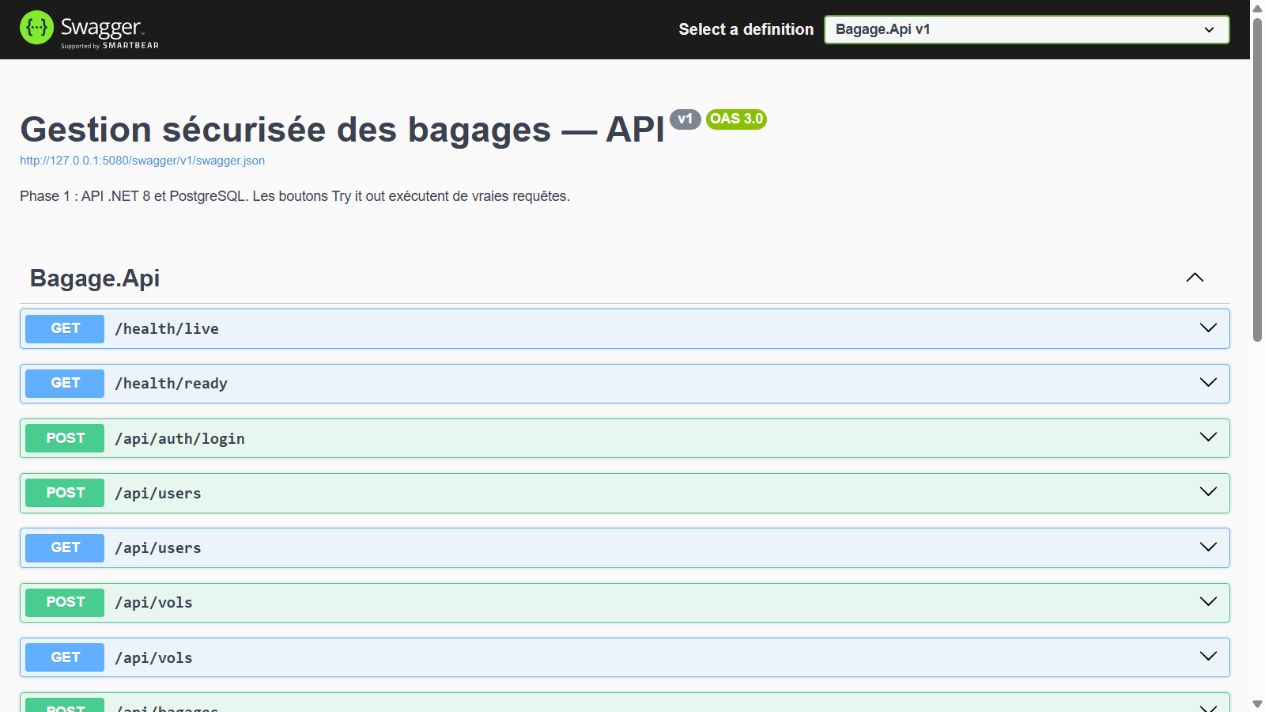
\includegraphics[width=0.96\linewidth,height=0.43\textheight,keepaspectratio]{../docs/captures/phase-01/01-api-routes.jpg}
\caption{Routes exposées par Swagger}
\label{fig:phase-01-1}
\end{figure}

\begin{figure}[!htbp]
\centering
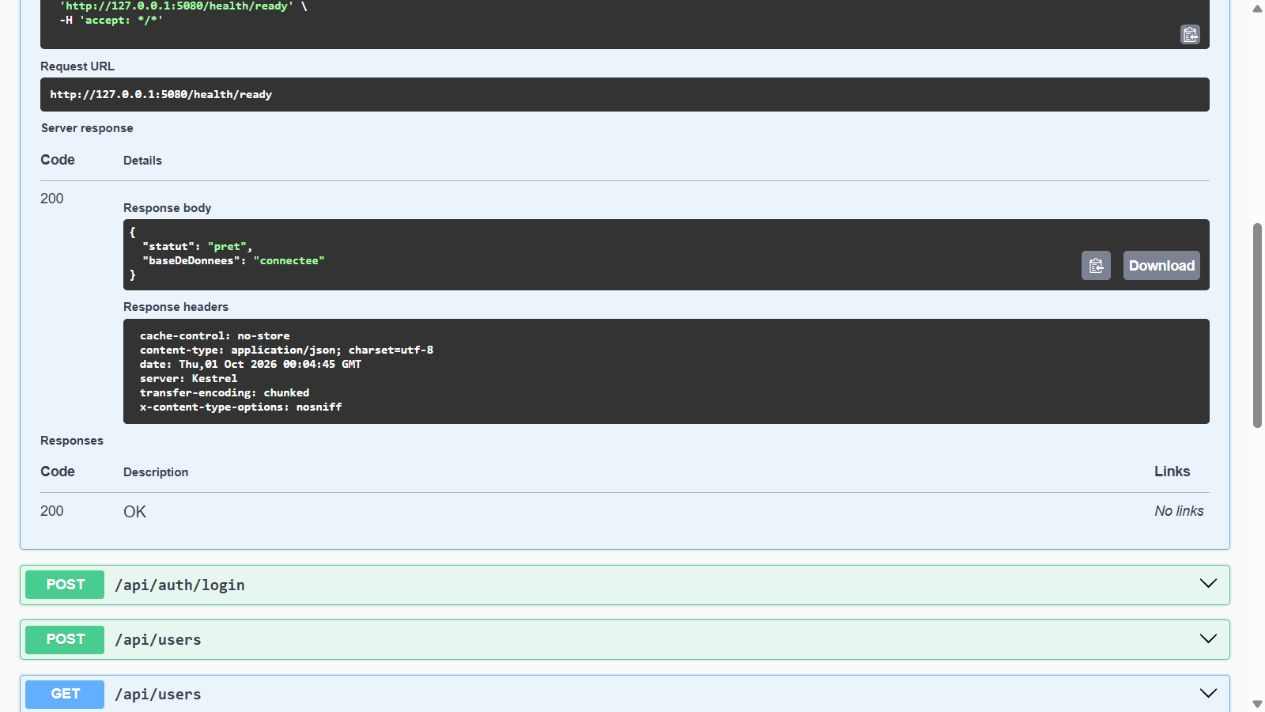
\includegraphics[width=0.96\linewidth,height=0.43\textheight,keepaspectratio]{../docs/captures/phase-01/02-postgresql-connecte.jpg}
\caption{Disponibilité de la connexion PostgreSQL}
\label{fig:phase-01-2}
\end{figure}

La liste des routes permet de repérer les fonctions disponibles, tandis que la réponse 200 de la sonde de disponibilité confirme la connexion à PostgreSQL. Ces deux observations valident le point de départ technique ; elles ne démontrent pas encore la sécurité des opérations.

\subsubsection{Distinguer lecture publique et opérations authentifiées}

Le suivi passager doit fonctionner sans compte, mais la consultation des vols relève des opérations internes. Cette différence est vérifiée directement dans l’API : un appel aux vols sans jeton est refusé, puis le code fictif de suivi permet de lire un parcours déjà enregistré.

\begin{figure}[!htbp]
\centering
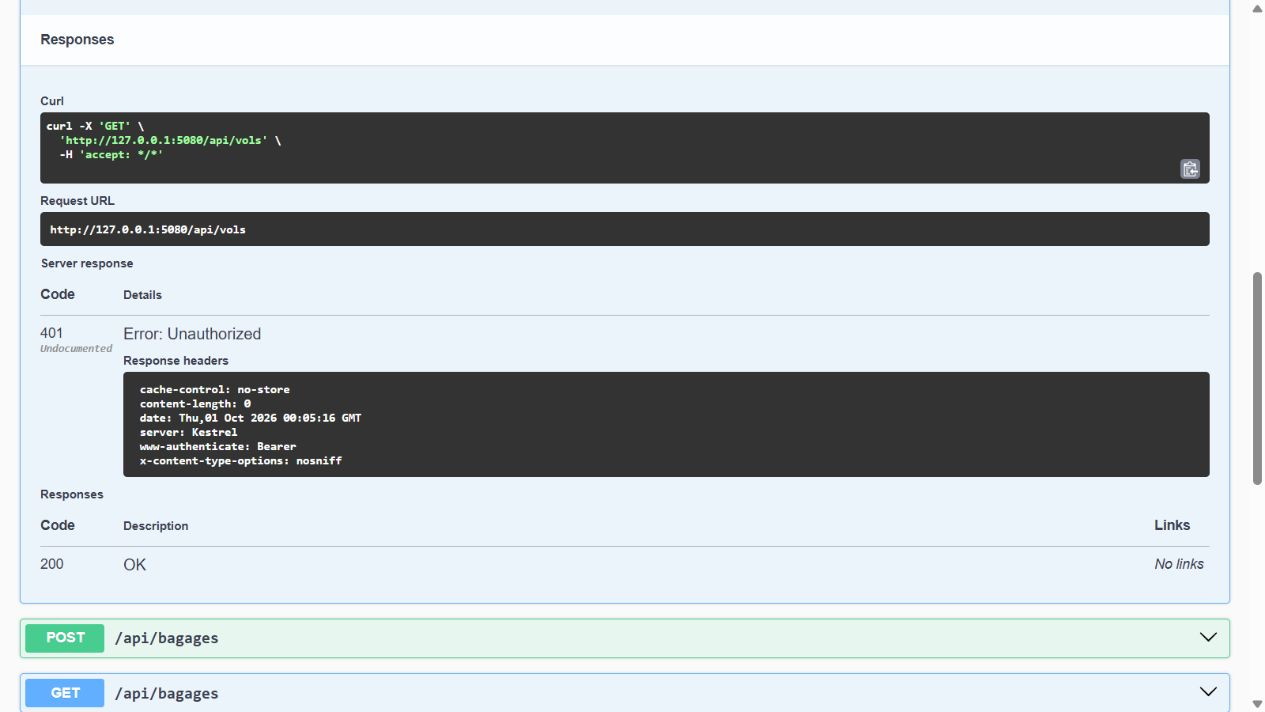
\includegraphics[width=0.96\linewidth,height=0.43\textheight,keepaspectratio]{../docs/captures/phase-01/03-acces-refuse-401.jpg}
\caption{Refus d’une requête sans JWT}
\label{fig:phase-01-3}
\end{figure}

\begin{figure}[!htbp]
\centering
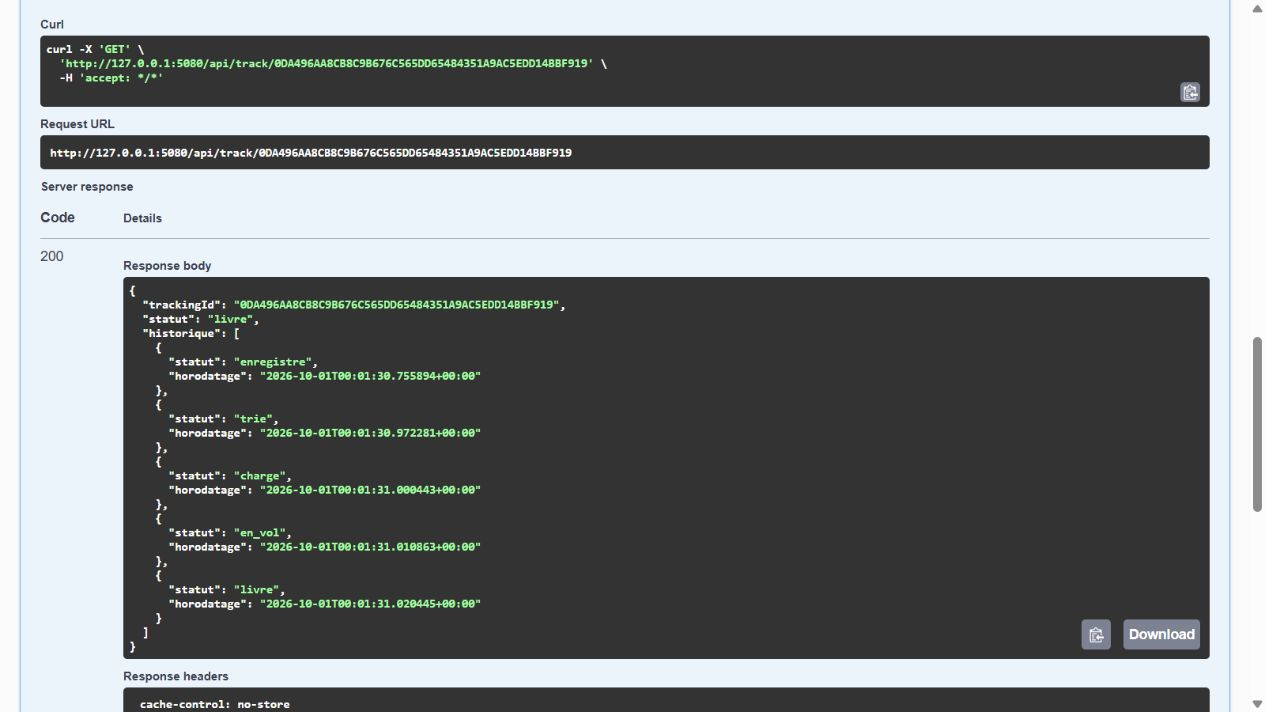
\includegraphics[width=0.96\linewidth,height=0.43\textheight,keepaspectratio]{../docs/captures/phase-01/04-tracking-public.jpg}
\caption{Suivi public fourni par l’API}
\label{fig:phase-01-4}
\end{figure}

La figure~\ref{fig:phase-01-3} vérifie le refus sans JWT, tandis que la figure~\ref{fig:phase-01-4} vérifie le maintien de la lecture publique. Le refus 401 est le résultat attendu de l’authentification applicative. La réponse de suivi présente le statut et les événements sans révéler l’identité du passager. La séparation fonctionnelle est donc établie avant l’ajout du VPN.

\subsubsection{Rendre l’exécution reproductible avec Docker}

L’API et PostgreSQL sont ensuite exécutés dans des conteneurs pour stabiliser leur environnement. Docker Desktop permet d’observer les deux services. La sonde de vie et le suivi sont rejoués sur l’API conteneurisée afin de vérifier que le changement d’environnement conserve le fonctionnement métier.

\begin{figure}[!htbp]
\centering
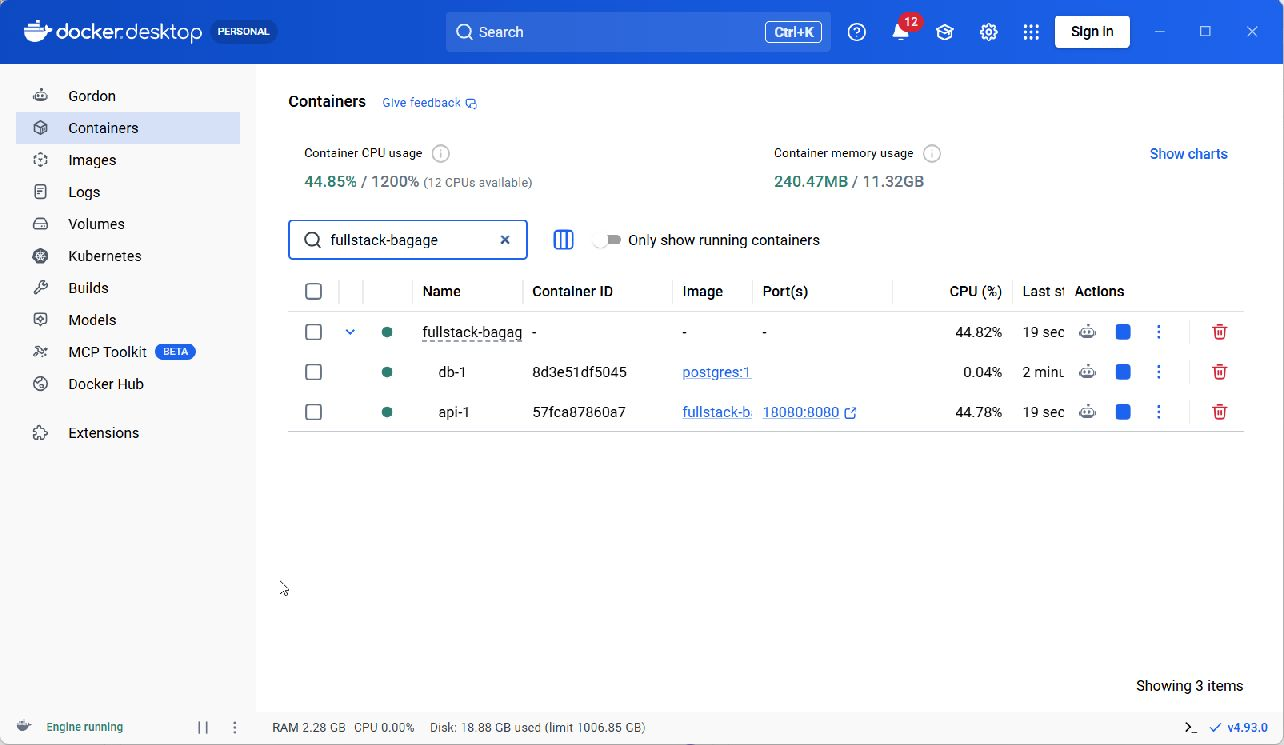
\includegraphics[width=0.96\linewidth,height=0.43\textheight,keepaspectratio]{../docs/captures/phase-01/05-docker-desktop.jpg}
\caption{Services de fondation dans Docker Desktop}
\label{fig:phase-01-5}
\end{figure}

\begin{figure}[!htbp]\centering
\begin{minipage}[t]{0.48\linewidth}\vspace{0pt}\centering
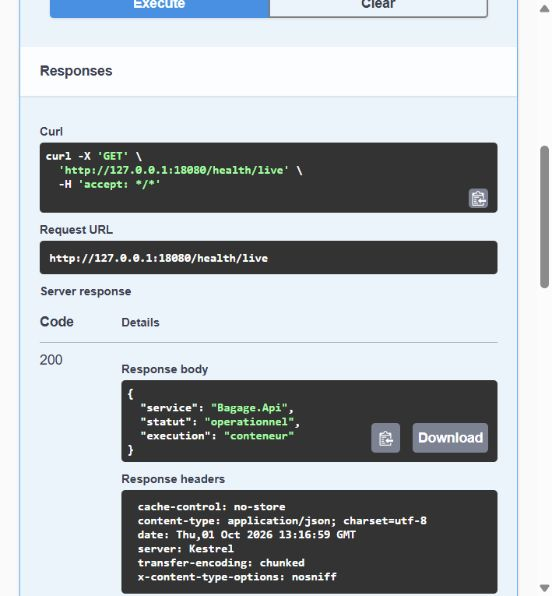
\includegraphics[width=\linewidth]{../docs/captures/phase-01/06-api-conteneur.jpg}
\caption{Exécution de l’API dans un conteneur}
\label{fig:phase-01-6}
\end{minipage}\hfill
\begin{minipage}[t]{0.48\linewidth}\vspace{0pt}\centering
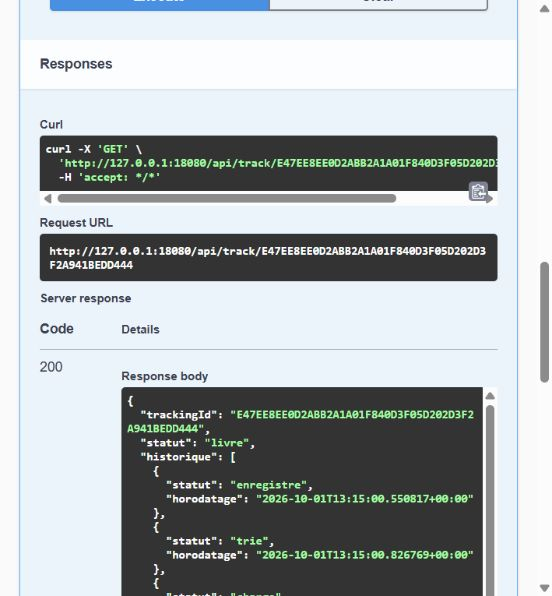
\includegraphics[width=\linewidth]{../docs/captures/phase-01/07-tracking-docker.jpg}
\caption{Suivi et historique depuis Docker}
\label{fig:phase-01-7}
\end{minipage}
\end{figure}

Les réponses restent cohérentes avec l’exécution native. Le port local 18080 appartient à cette étape de développement ; les phases suivantes retireront la publication directe de l’API. La chaîne de données étant opérationnelle, le travail peut se poursuivre sur les interfaces utilisateur.

\FloatBarrier
\subsection{Interfaces Angular : réaliser un parcours métier complet}

\subsubsection{Préparer les accès public et agents}

Deux applications Angular sont compilées séparément. L’accueil public propose uniquement la recherche par code. L’espace agents possède une navigation privée ; lorsque la page des bagages est demandée sans session, la garde conduit vers la connexion. Cette séparation rend visibles les deux usages dès l’entrée dans l’application.

\begin{figure}[!htbp]
\centering
\begin{minipage}[t]{0.58\linewidth}\vspace{0pt}\centering
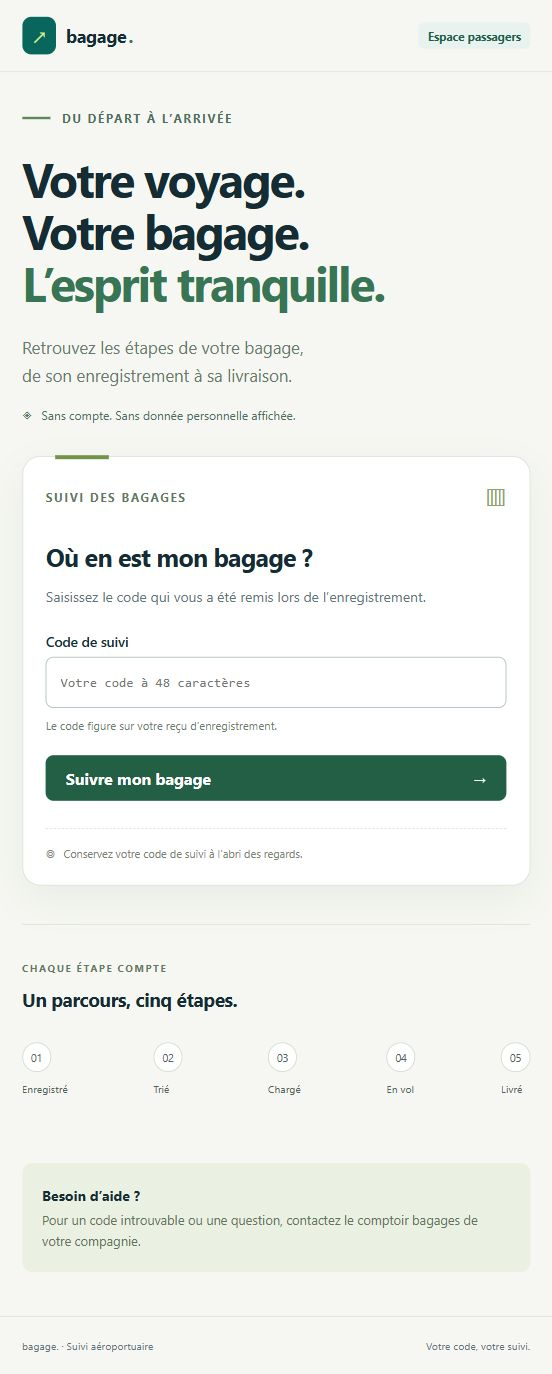
\includegraphics[width=\linewidth,trim=0bp 474bp 0bp 0bp,clip]{../docs/captures/phase-02/01-accueil-public.jpg}
\end{minipage}\hfill
\begin{minipage}[t]{0.38\linewidth}\vspace{0pt}\centering
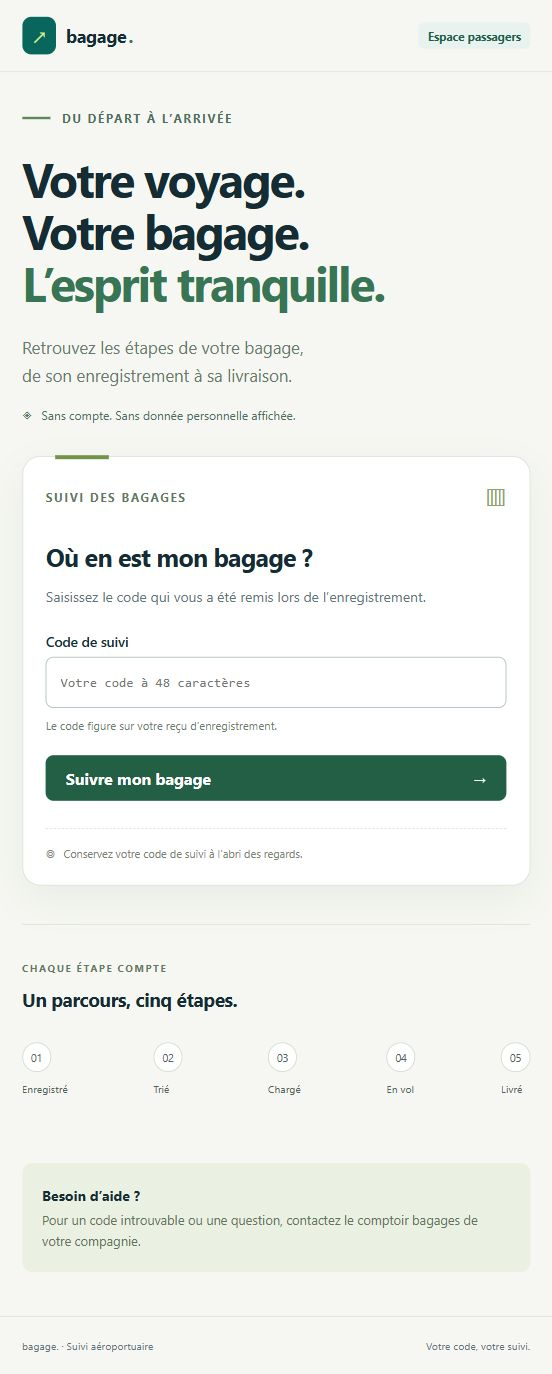
\includegraphics[width=\linewidth,trim=0bp 0bp 0bp 900bp,clip]{../docs/captures/phase-02/01-accueil-public.jpg}
\end{minipage}
\caption{Accueil public du suivi passager : formulaire à gauche et suite de la page à droite}
\label{fig:phase-02-1}
\end{figure}

\begin{figure}[!htbp]
\centering
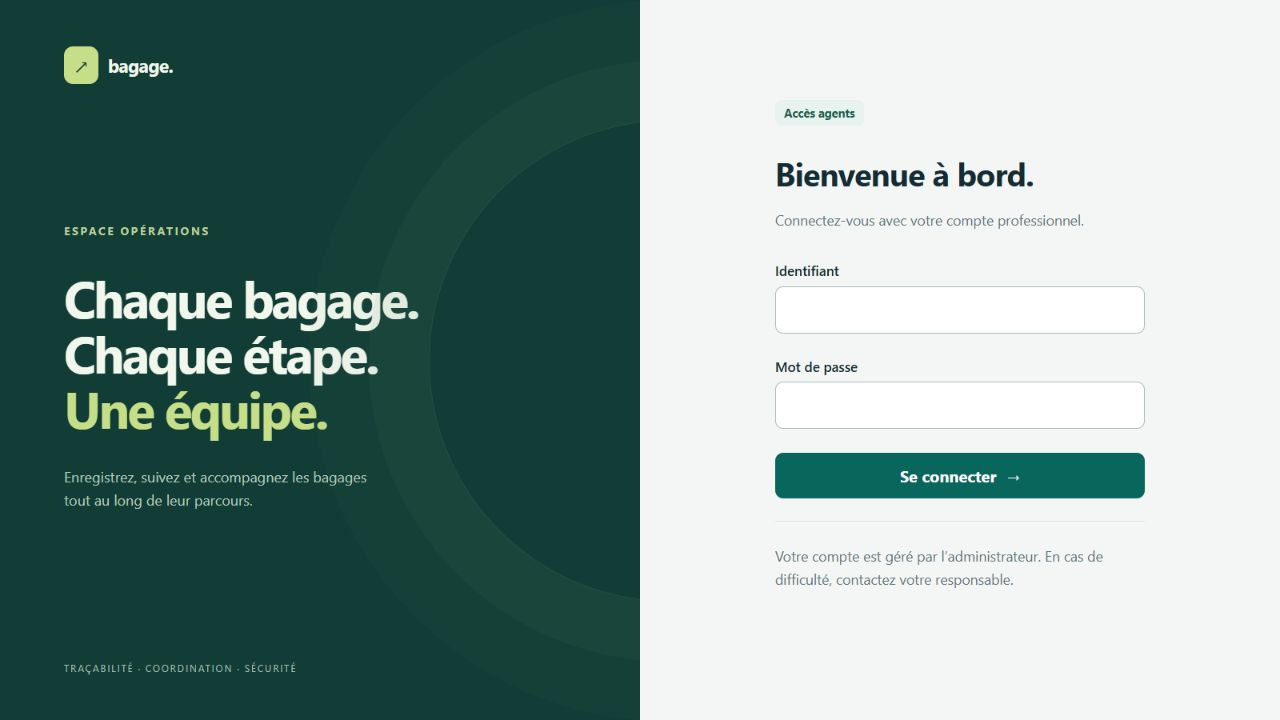
\includegraphics[width=0.96\linewidth,height=0.43\textheight,keepaspectratio]{../docs/captures/phase-02/03-connexion-agents.jpg}
\caption{Redirection vers la connexion agents}
\label{fig:phase-02-3}
\end{figure}

La figure~\ref{fig:phase-02-1} répond au besoin de consultation sans compte ; la figure~\ref{fig:phase-02-3} matérialise le point d'entrée réservé aux agents. Le passager n’a pas à s’authentifier pour utiliser son code. L’agent doit ouvrir une session avant les fonctions internes. Cette protection de navigation accompagne les contrôles de l’API ; elle ne les remplace pas.

\subsubsection{Organiser le travail du superviseur}

Le superviseur dispose d’une vue métier des bagages et des vols. Les indicateurs du tableau de bord sont calculés à partir des listes chargées et sont présentés avec leurs limites. Ce rôle prépare le contexte de l’enregistrement et ne donne pas automatiquement accès à la gestion des comptes.

\begin{figure}[!htbp]
\centering
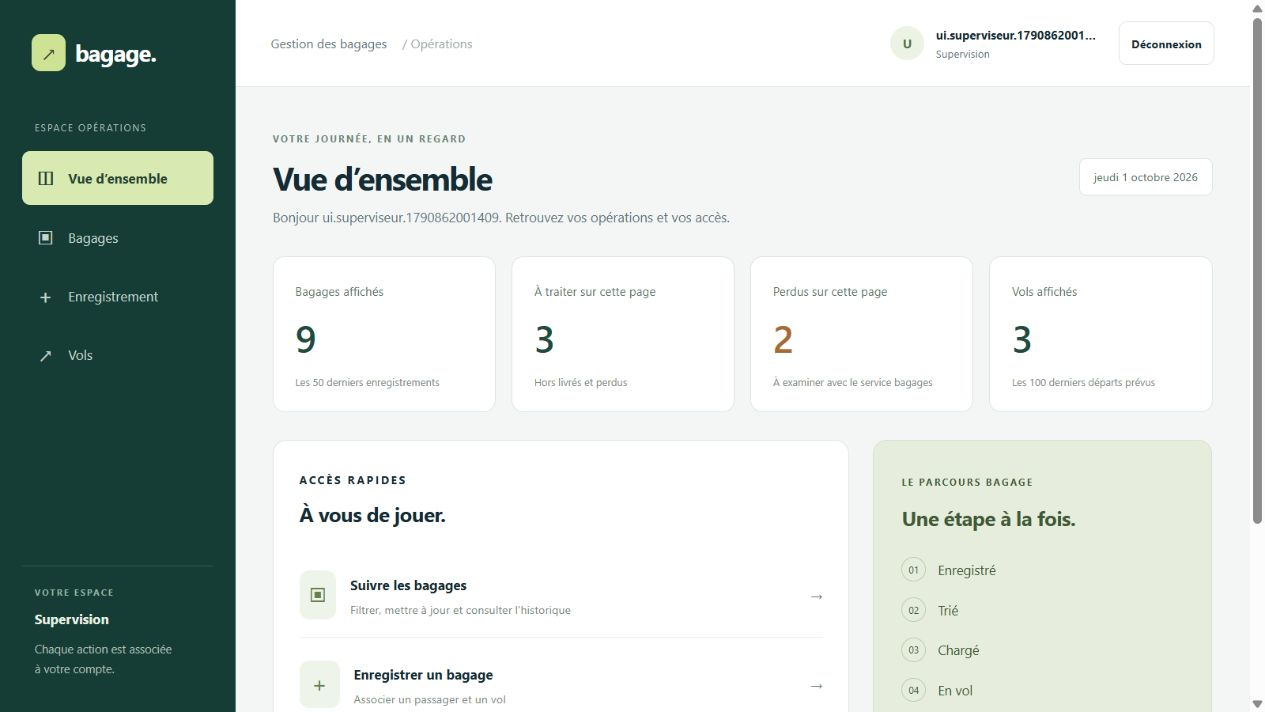
\includegraphics[width=0.96\linewidth,height=0.43\textheight,keepaspectratio]{../docs/captures/phase-02/04-dashboard-superviseur.jpg}
\caption{Tableau de bord du superviseur}
\label{fig:phase-02-4}
\end{figure}

La capture montre les menus métier accessibles au superviseur et l’absence du menu comptes. La distinction des responsabilités est ainsi visible dans l’interface avant d’être contrôlée lors des appels API.

\subsubsection{Enregistrer le bagage puis effectuer le tri}

Après création du vol, l’agent d’enregistrement sélectionne ce vol et saisit les données fictives du bagage. La création produit un reçu et un code de suivi. L’agent de tri retrouve ensuite le bagage et demande le passage à l’étape Trié ; l’API contrôle la transition et ajoute l’événement associé.

\begin{figure}[!htbp]
\centering
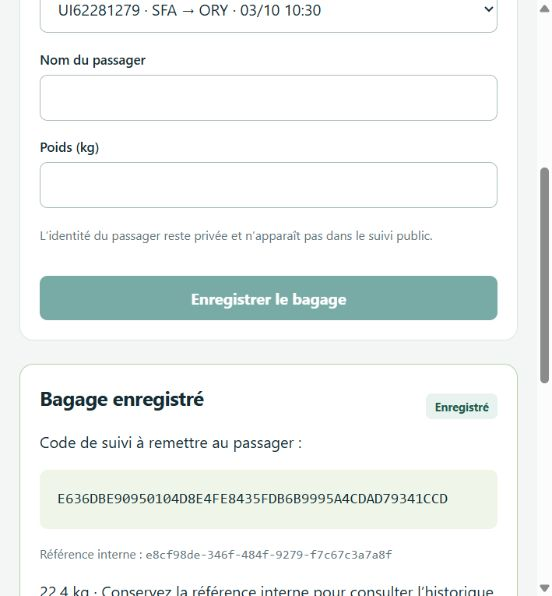
\includegraphics[width=0.62\linewidth,height=0.43\textheight,keepaspectratio]{../docs/captures/phase-02/06-enregistrement-recu.jpg}
\caption{Enregistrement et reçu de suivi}
\label{fig:phase-02-6}
\end{figure}

\begin{figure}[!htbp]
\centering
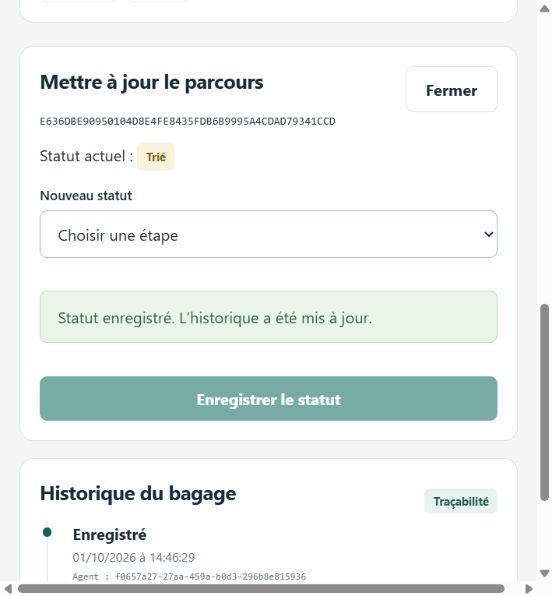
\includegraphics[width=0.62\linewidth,height=0.43\textheight,keepaspectratio]{../docs/captures/phase-02/07-role-tri.jpg}
\caption{Transition effectuée par l’agent de tri}
\label{fig:phase-02-7}
\end{figure}

Le reçu relie l’opération interne au suivi passager. L’historique de tri montre que le statut n’est pas une simple modification d’affichage : il correspond à une transition conservée en base. Le passager peut maintenant consulter ce parcours.

\subsubsection{Vérifier la continuité avec le suivi passager}

Le code obtenu lors de l’enregistrement est saisi dans l’application publique. La consultation restitue l’état Trié et les horodatages du parcours. Les données viennent de la même API et de la même base que celles utilisées par les agents.

\begin{figure}[!htbp]
\centering
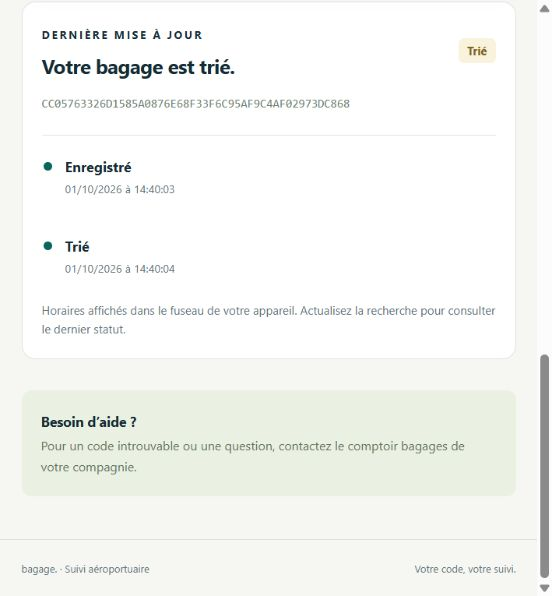
\includegraphics[width=0.62\linewidth,height=0.43\textheight,keepaspectratio]{../docs/captures/phase-02/02-suivi-public.jpg}
\caption{Consultation du statut Trié}
\label{fig:phase-02-2}
\end{figure}

Cette étape ferme la boucle entre enregistrement, manutention et information du passager. La capture reflète l’état du bagage au moment de la consultation ; une correction ultérieure peut modifier ce statut sans invalider la trace historique de cette étape.

\subsubsection{Conserver la trace des corrections exceptionnelles}

Une transition qui sort du parcours normal demande l’intervention du superviseur et un motif. Le scénario de correction vers Livré vérifie que l’application conserve la justification et l’agent responsable, au lieu de masquer l’anomalie par un changement silencieux.

\begin{figure}[!htbp]
\centering
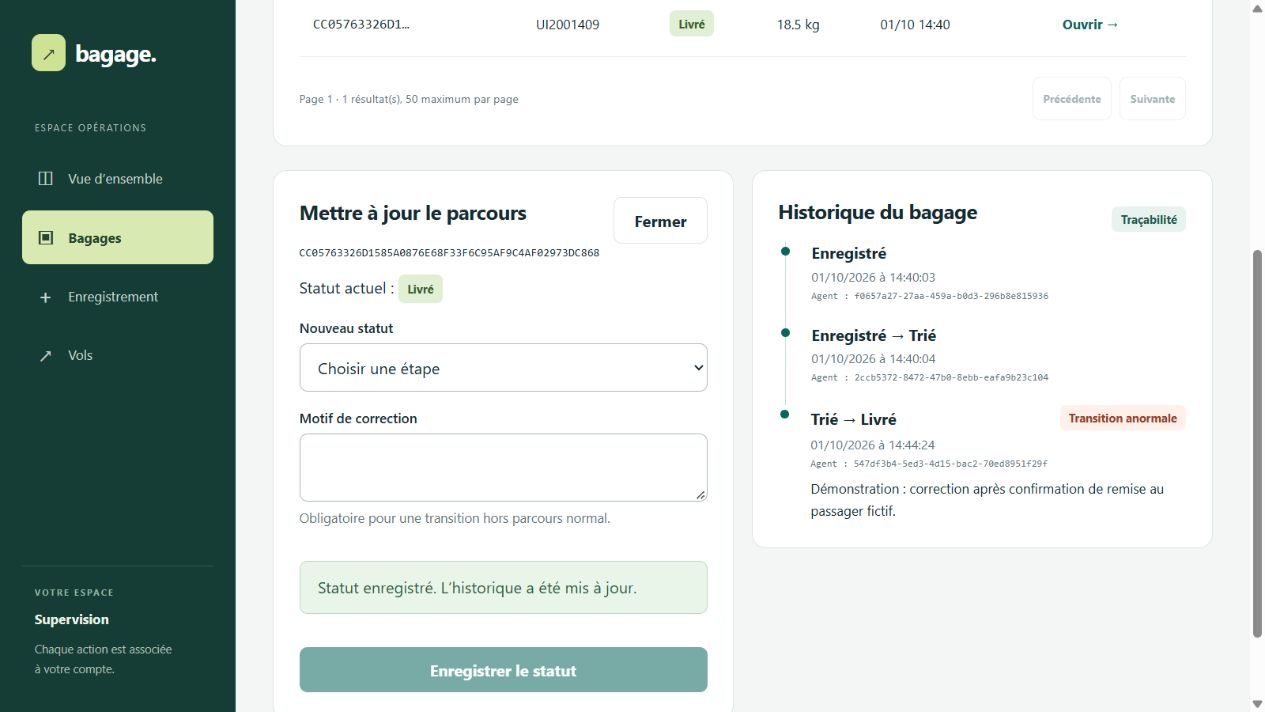
\includegraphics[width=0.96\linewidth,height=0.43\textheight,keepaspectratio]{../docs/captures/phase-02/05-anomalie-historique.jpg}
\caption{Correction exceptionnelle et historique}
\label{fig:phase-02-5}
\end{figure}

L’événement marqué comme exceptionnel permet de comprendre la correction. La traçabilité reste donc exploitable même lorsque le cycle normal n’a pas été suivi intégralement.

\subsubsection{Isoler l’administration et contrôler l’origine de l’interface}

Le compte administrateur est réservé à la gestion des utilisateurs. Une création de compte fictif est réalisée depuis son formulaire. L’application agents vérifie aussi son origine de service : une origine locale absente de la liste autorisée empêche le chargement du module.

\begin{figure}[!htbp]
\centering
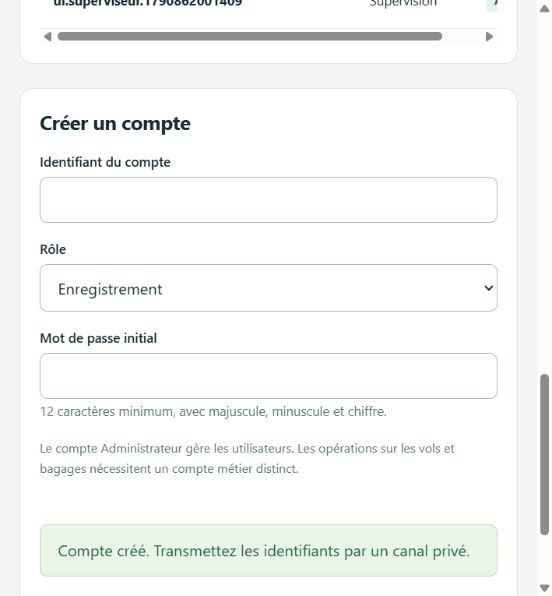
\includegraphics[width=0.62\linewidth,height=0.43\textheight,keepaspectratio]{../docs/captures/phase-02/08-creation-compte.jpg}
\caption{Création d’un compte par l’administrateur}
\label{fig:phase-02-8}
\end{figure}

\begin{figure}[!htbp]
\centering
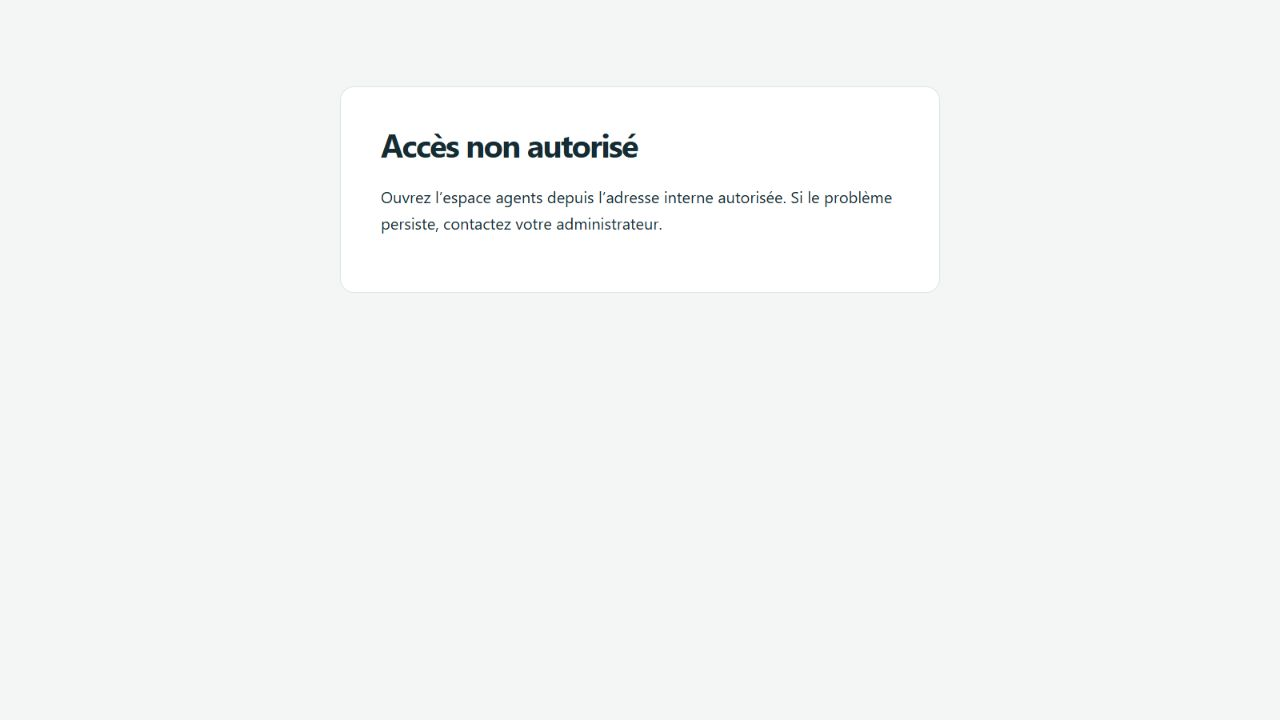
\includegraphics[width=0.96\linewidth,height=0.43\textheight,keepaspectratio]{../docs/captures/phase-02/09-origine-refusee.jpg}
\caption{Contrôle applicatif de l’origine}
\label{fig:phase-02-9}
\end{figure}

La confirmation de création ne révèle pas le mot de passe. Le refus d’origine constitue un contrôle applicatif supplémentaire, distinct du VPN. Les parcours ayant été vérifiés, la réalisation aborde maintenant la protection réseau nécessaire aux opérations privées.

\FloatBarrier
\subsection{Sécurisation réseau : ajouter le VPN aux autorisations applicatives}

\subsubsection{Segmenter les conteneurs et limiter les publications}

Les composants sont répartis sur des réseaux dédiés au point d’entrée, aux échanges avec l’API et à PostgreSQL. Nginx public relaie uniquement le suivi ; le proxy agents reste sur le chemin privé. WireGuard ajoute la passerelle nécessaire aux clients habilités. La vue Docker Desktop permet de vérifier l’organisation obtenue.

\begin{figure}[!htbp]
\centering
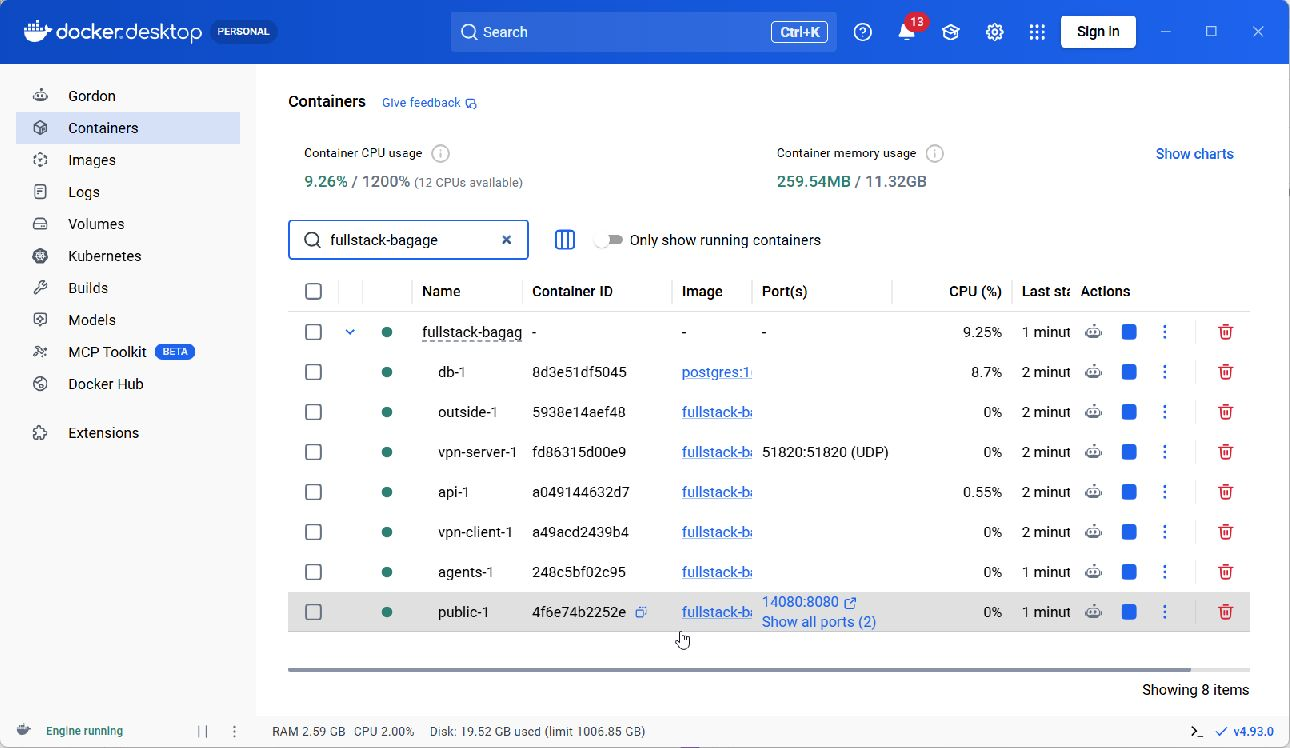
\includegraphics[width=0.96\linewidth,height=0.43\textheight,keepaspectratio]{../docs/captures/phase-03/01-reseau-conteneurs.jpg}
\caption{Organisation des conteneurs réseau}
\label{fig:phase-03-1}
\end{figure}

La présence des services ne signifie pas que leurs ports sont accessibles à tous. Les fonctions privées ne sont plus publiées comme dans le laboratoire initial. Il reste à vérifier cette frontière depuis des clients placés avec et sans tunnel.

\subsubsection{Tester le tunnel avec le même jeton}

Un client autorisé établit le tunnel puis utilise un JWT valide pour atteindre le service privé. Le tunnel est coupé en conservant ce jeton, puis rétabli. Un second client, extérieur au VPN dans le laboratoire Docker, essaie les mêmes accès et consulte le suivi public.

\begin{figure}[!htbp]
\centering
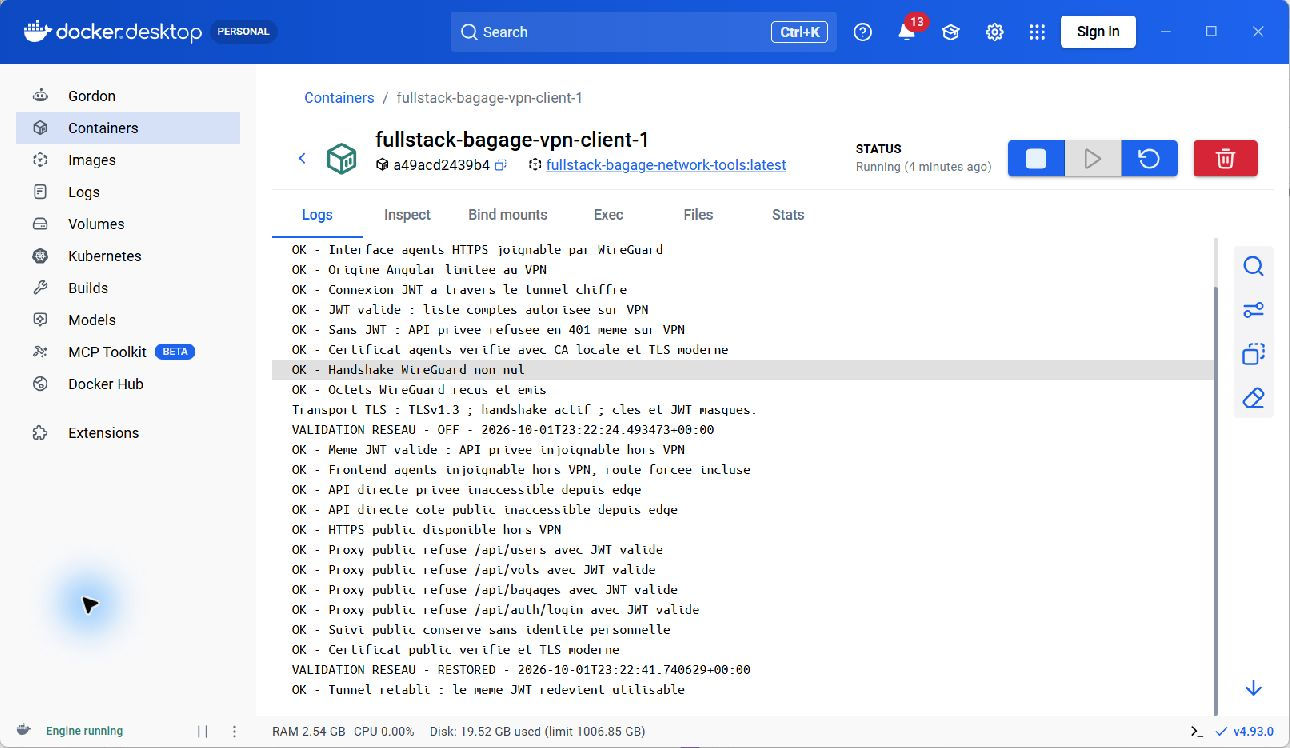
\includegraphics[width=0.96\linewidth,height=0.43\textheight,keepaspectratio,trim=162bp 19.2bp 33bp 117bp,clip]{../docs/captures/phase-03/02-vpn-coupure-retablissement.jpg}
\caption{Accès privé, coupure et rétablissement du tunnel}
\label{fig:phase-03-2}
\end{figure}

\begin{figure}[!htbp]
\centering
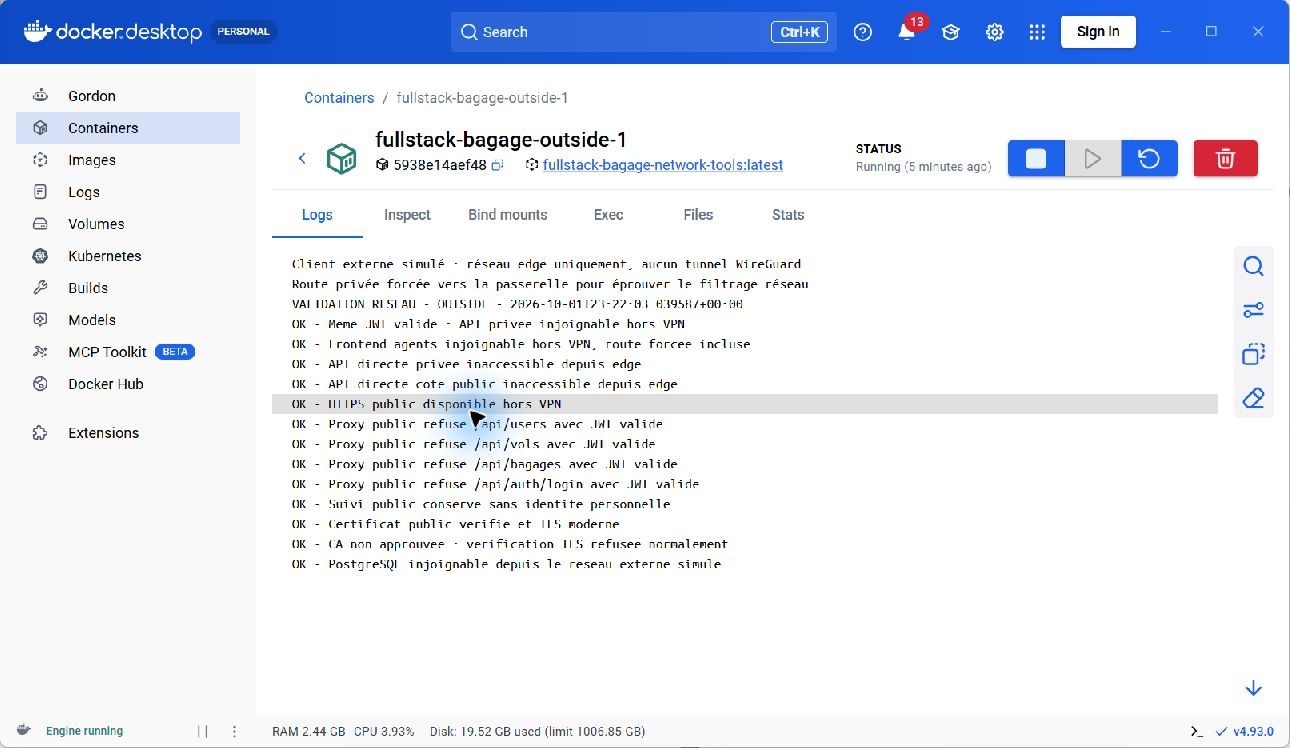
\includegraphics[width=0.96\linewidth,height=0.43\textheight,keepaspectratio,trim=162bp 19.2bp 33bp 117bp,clip]{../docs/captures/phase-03/03-acces-hors-vpn.jpg}
\caption{Client extérieur au VPN dans le laboratoire}
\label{fig:phase-03-3}
\end{figure}

La figure~\ref{fig:phase-03-2} isole l'effet du VPN en conservant le même JWT ; la figure~\ref{fig:phase-03-3} complète cette preuve depuis un client extérieur au tunnel. L’accès privé disparaît à la coupure et revient avec le tunnel, tandis que le site public reste disponible. Ce résultat montre que le JWT ne suffit pas à franchir la frontière réseau. À cette étape, les clients sont encore des conteneurs sur le même poste : la validation porte sur le laboratoire, avant son transfert vers Kubernetes.

\FloatBarrier
\subsection{Kubernetes : déployer les composants et vérifier la persistance}

\subsubsection{Installer le cluster et déclarer les ressources}

Un cluster k3s mono-nœud est créé dans k3d. L’API et les interfaces utilisent des Deployments ; PostgreSQL utilise un StatefulSet et un volume persistant. Les migrations et l’initialisation passent par des Jobs. Les sorties kubectl enregistrées complètent la vue du nœud dans Docker Desktop.

\begin{figure}[!htbp]
\centering
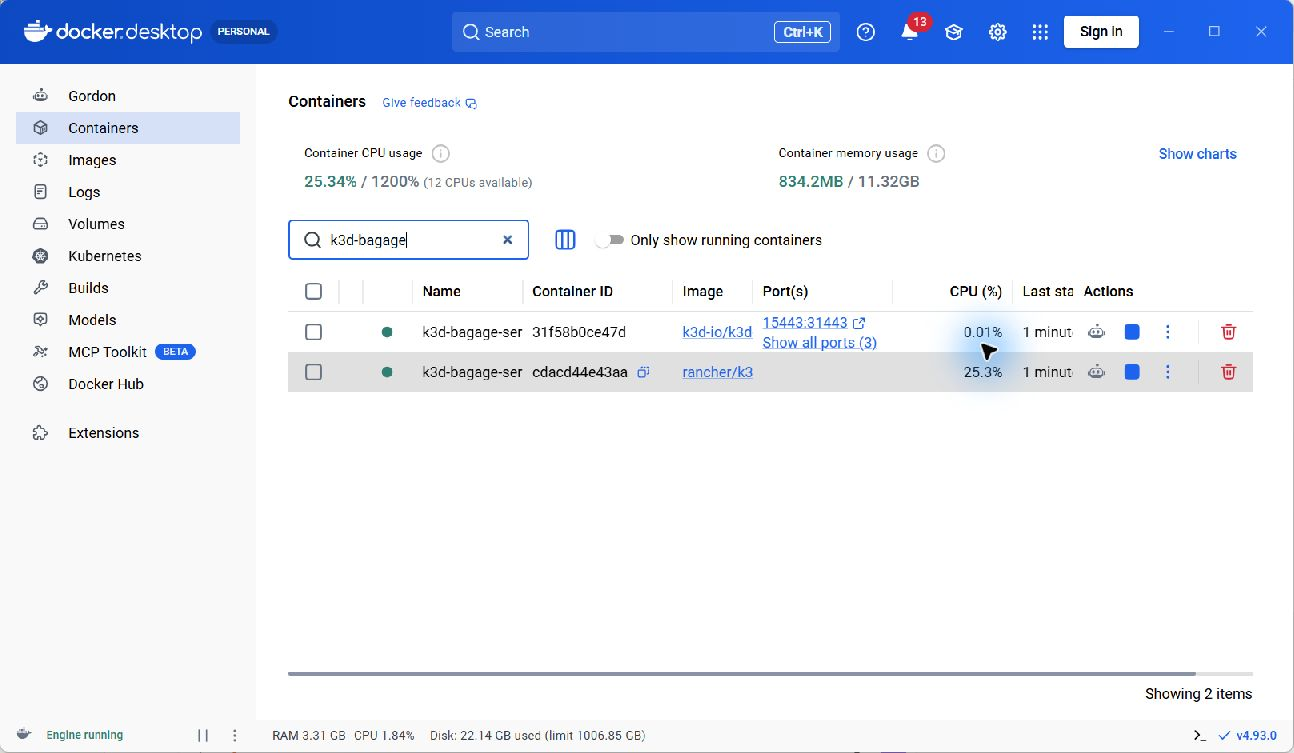
\includegraphics[width=0.96\linewidth,height=0.43\textheight,keepaspectratio]{../docs/captures/phase-04/01-cluster-k3s.jpg}
\caption{Cluster k3s dans k3d}
\label{fig:phase-04-1}
\end{figure}

\begin{figure}[!htbp]
\centering
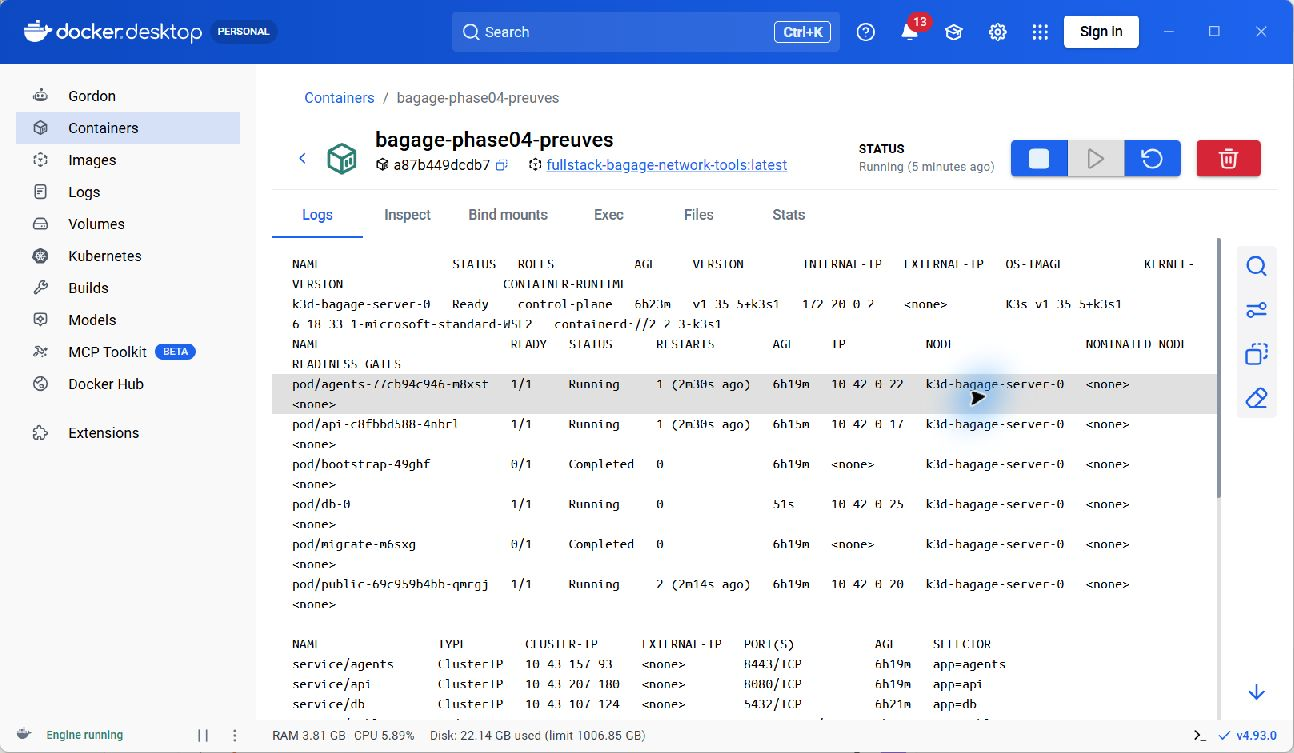
\includegraphics[width=0.96\linewidth,height=0.43\textheight,keepaspectratio]{../docs/captures/phase-04/04-ressources-kubernetes.jpg}
\caption{Ressources observées avec kubectl}
\label{fig:phase-04-4}
\end{figure}

Le lecteur de sorties kubectl visible dans Docker sert uniquement à consulter les preuves. Les services privés sont déclarés en ClusterIP, les flux sont limités par NetworkPolicy et le stockage reste local au nœud. Le déploiement doit ensuite être vérifié depuis ses points d’entrée.

\subsubsection{Retrouver les protections réseau et conserver les données}

Les essais avec et sans VPN sont reproduits contre Kubernetes. La validation contrôle également les politiques réseau et le remplacement du pod PostgreSQL. Après ce remplacement, le bagage et ses événements doivent rester disponibles grâce au volume persistant.

\begin{figure}[!htbp]
\centering
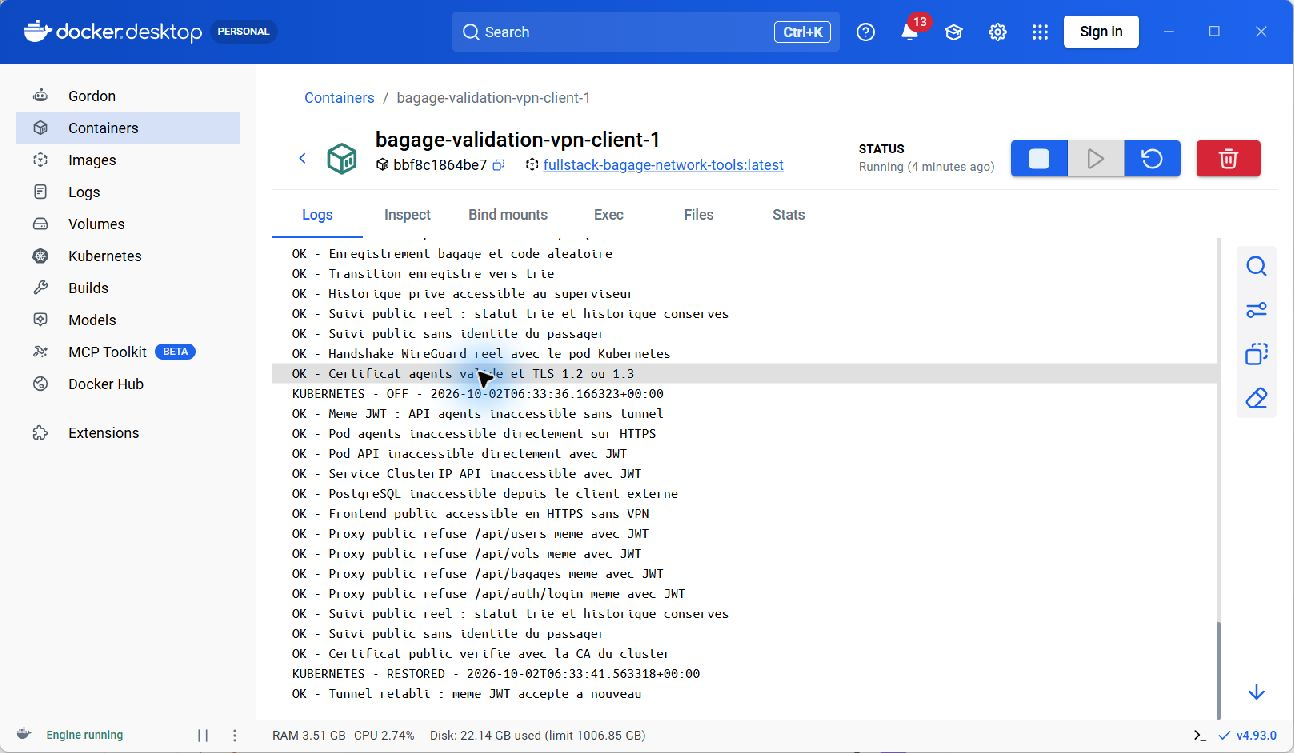
\includegraphics[width=0.96\linewidth,height=0.43\textheight,keepaspectratio,trim=162bp 19.2bp 33bp 117bp,clip]{../docs/captures/phase-04/02-vpn-kubernetes.jpg}
\caption{WireGuard et services privés du cluster}
\label{fig:phase-04-2}
\end{figure}

\begin{figure}[!htbp]
\centering
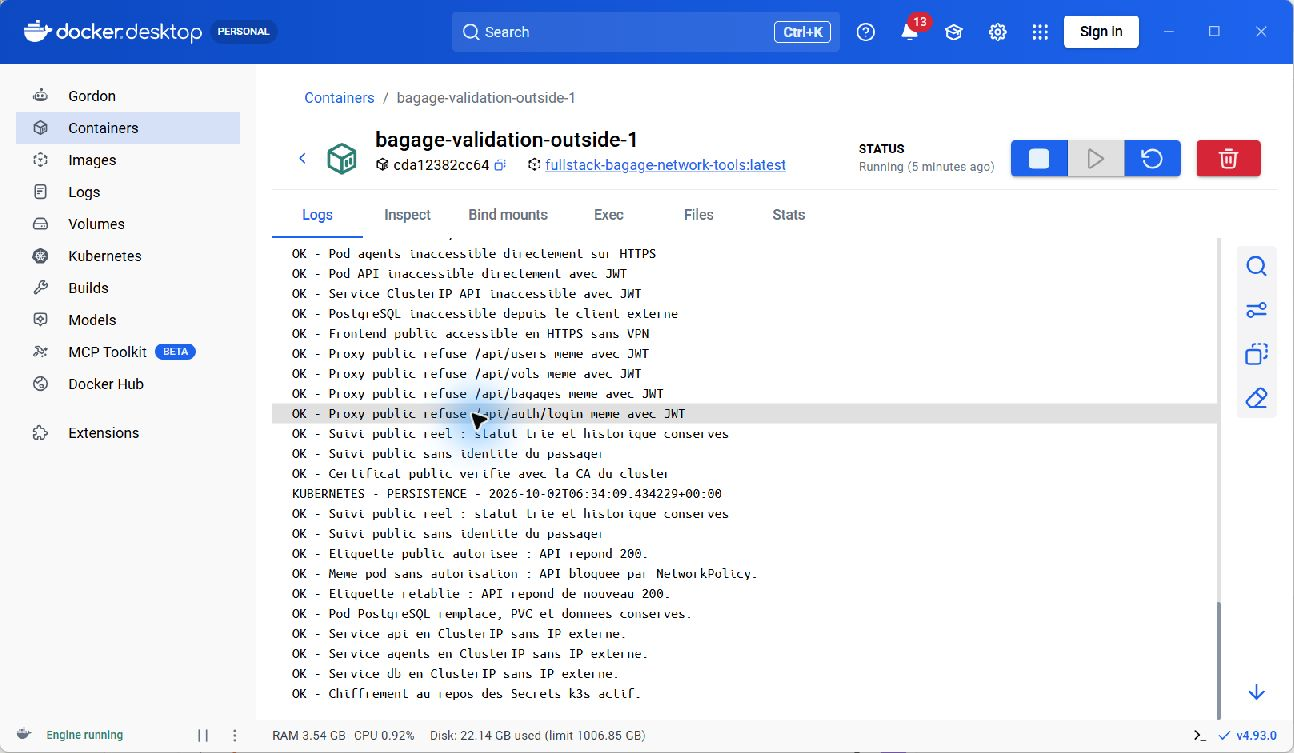
\includegraphics[width=0.96\linewidth,height=0.43\textheight,keepaspectratio,trim=162bp 19.2bp 33bp 117bp,clip]{../docs/captures/phase-04/03-hors-vpn-persistance.jpg}
\caption{Restrictions et persistance Kubernetes}
\label{fig:phase-04-3}
\end{figure}

La frontière VPN est conservée après le changement de mode de déploiement. La persistance vérifiée concerne le remplacement du pod ; elle ne prouve pas une reprise après perte du disque. Une restauration de sauvegarde sera donc testée séparément.

\subsubsection{Sortir du client Docker : Windows et Ubuntu VMware}

Le client WireGuard natif de Windows est utilisé pour vérifier le chemin réel du poste vers le service privé. Une VM Ubuntu exécute ensuite la même famille de contrôles. Les résultats de ces systèmes sont archivés puis consultés dans Docker Desktop, qui joue ici le rôle de lecteur et non celui de client testé.

\begin{figure}[!htbp]
\centering
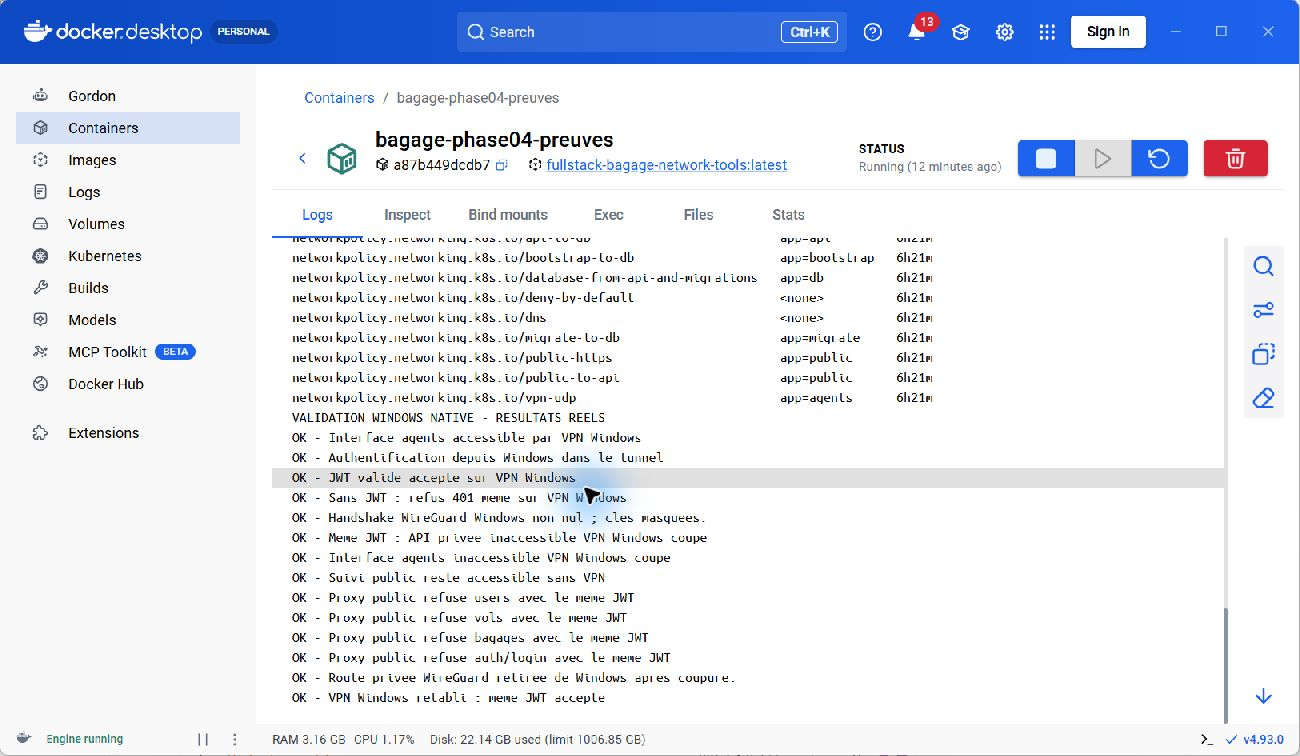
\includegraphics[width=0.96\linewidth,height=0.43\textheight,keepaspectratio,trim=162bp 19.2bp 33bp 117bp,clip]{../docs/captures/phase-04/05-vpn-windows-natif.jpg}
\caption{Validation avec le client Windows natif}
\label{fig:phase-04-5}
\end{figure}

\begin{figure}[!htbp]
\centering
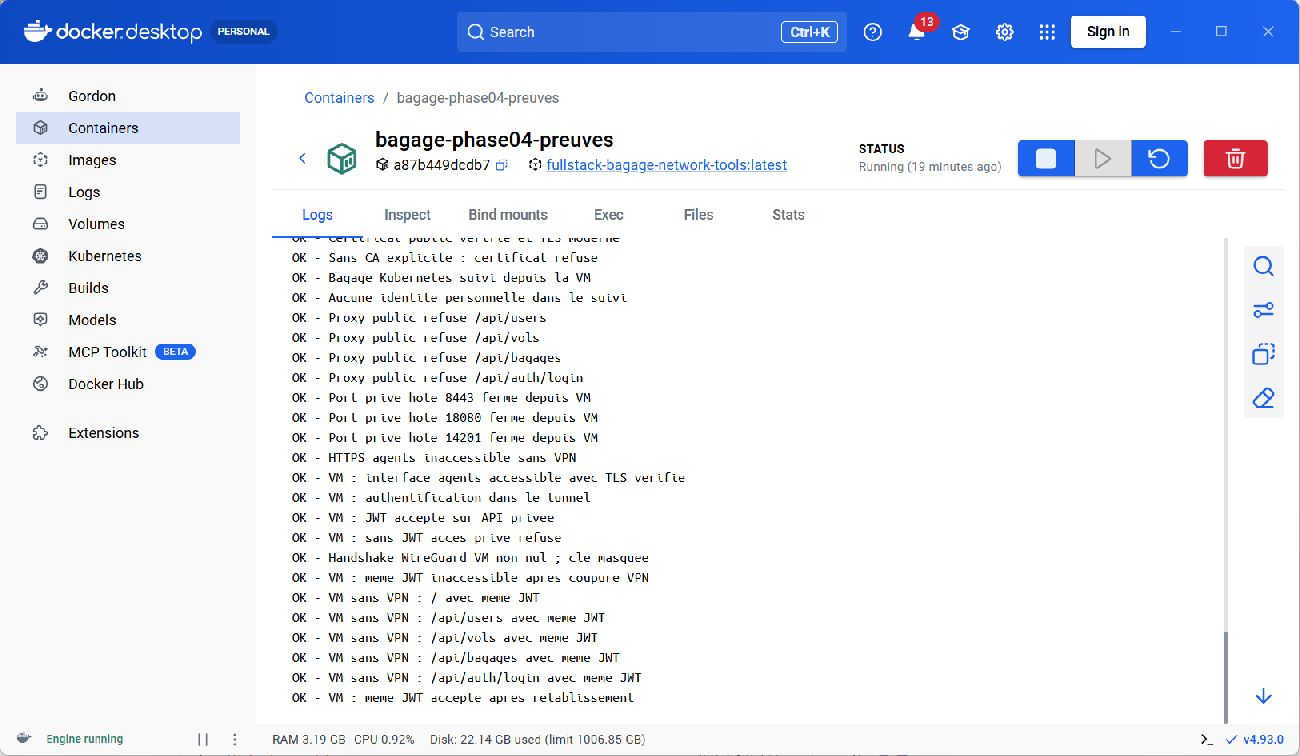
\includegraphics[width=0.96\linewidth,height=0.43\textheight,keepaspectratio,trim=162bp 19.2bp 33bp 117bp,clip]{../docs/captures/phase-04/06-validation-vmware.jpg}
\caption{Validation depuis Ubuntu VMware}
\label{fig:phase-04-6}
\end{figure}

Ces essais confirment le fonctionnement depuis Windows et un système invité Ubuntu. La VM reste sur le même poste physique : son utilisation ne suffit pas, à elle seule, à conclure à un accès VPN depuis Internet.

\subsubsection{Préparer une VM dédiée aux validations}

Une nouvelle VM est installée depuis l’ISO Ubuntu fourni, sur un disque distinct. Son premier démarrage confirme l’installation. Les tests réseau et VPN sont ensuite exécutés dans sa console, puis complétés par la consultation HTTPS du service public via une URL temporaire.

\begin{figure}[!htbp]
\centering
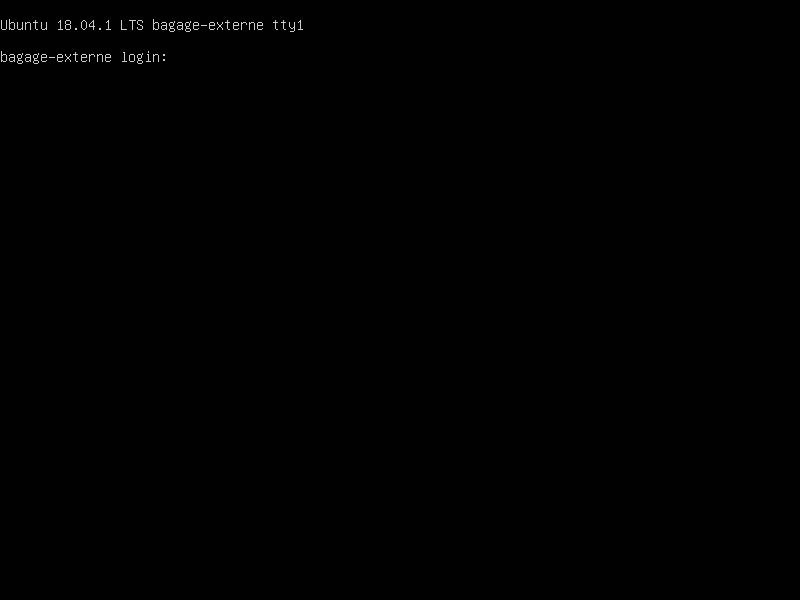
\includegraphics[width=0.96\linewidth,height=0.43\textheight,keepaspectratio,trim=0bp 524bp 485bp 7bp,clip]{../docs/captures/phase-04d/01-demarrage-ubuntu.png}
\caption{Premier démarrage de la VM Ubuntu}
\label{fig:phase-04d-1}
\end{figure}

\begin{figure}[!htbp]
\centering
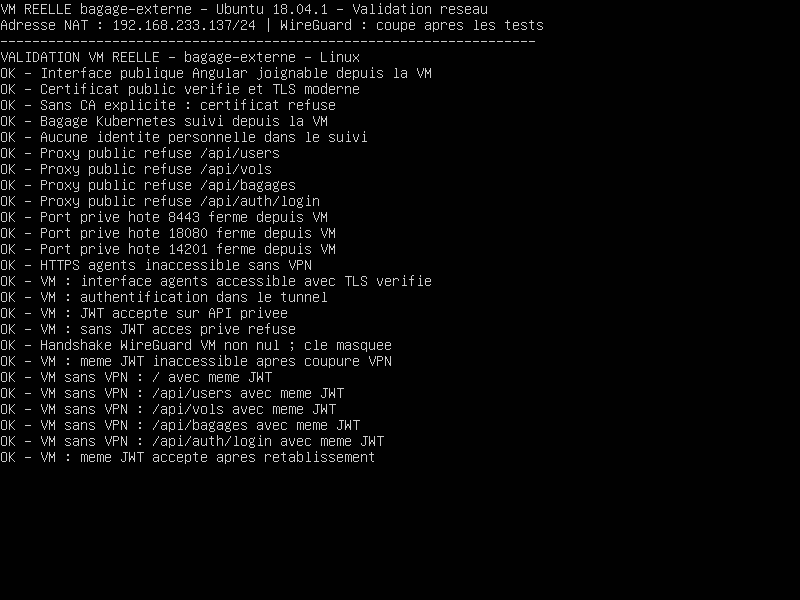
\includegraphics[width=0.96\linewidth,height=0.43\textheight,keepaspectratio,trim=0bp 124bp 245bp 0bp,clip]{../docs/captures/phase-04d/02-validation-vm.png}
\caption{Contrôles réseau et VPN dans la VM}
\label{fig:phase-04d-2}
\end{figure}

\begin{figure}[!htbp]
\centering
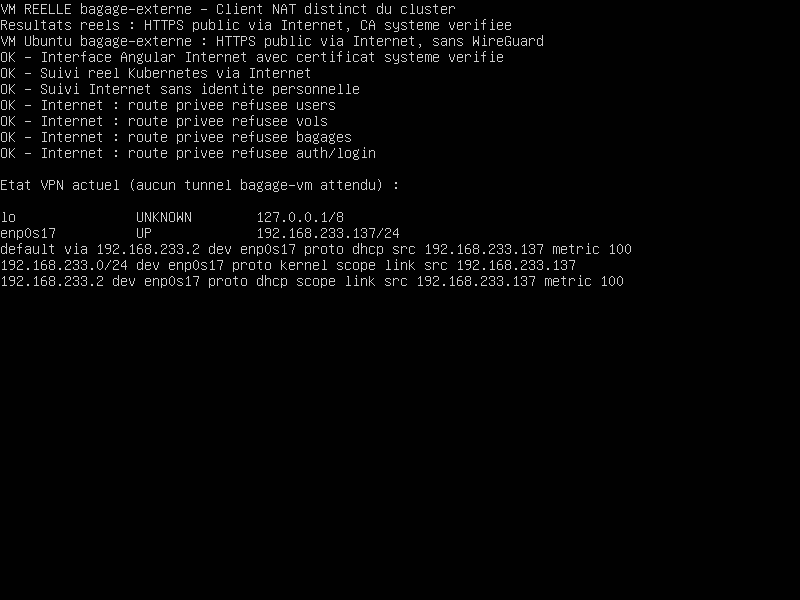
\includegraphics[width=0.96\linewidth,height=0.43\textheight,keepaspectratio,trim=0bp 300bp 157bp 0bp,clip]{../docs/captures/phase-04d/03-internet-vm.png}
\caption{HTTPS public depuis la VM dédiée}
\label{fig:phase-04d-3}
\end{figure}

La VM dédiée fournit un client de laboratoire reproductible. Les tests de tunnel local et les contrôles HTTPS publics sont distingués : seuls ces derniers empruntent l’URL Internet temporaire. La suite du travail examine séparément la fermeture des ports locaux et le tunnel Internet.

\subsubsection{Vérifier les ports du poste partagé}

Les services Windows étrangers au projet sont liés à localhost afin de ne plus les exposer sur le LAN. Depuis la seconde VM, les ports concernés sont contrôlés, puis les accès par VPN local et les restrictions du site public sont vérifiés.

\begin{figure}[!htbp]
\centering
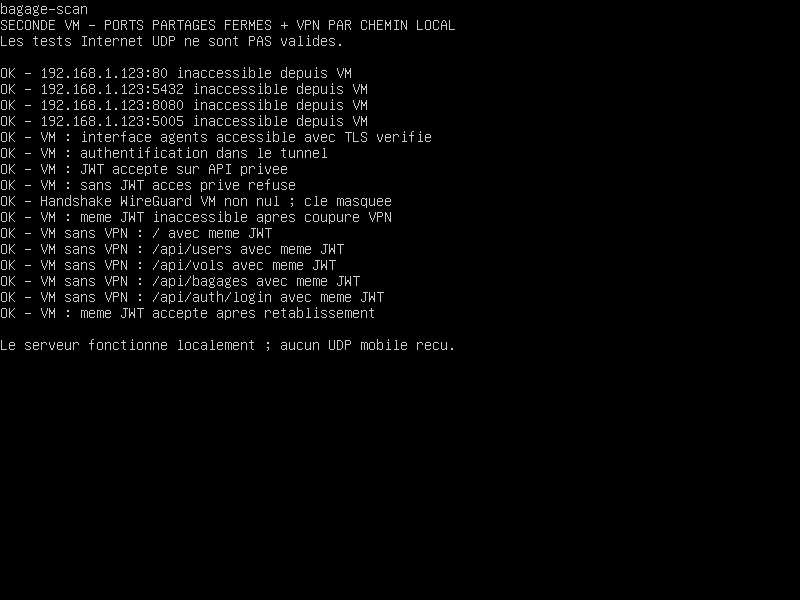
\includegraphics[width=0.96\linewidth,height=0.43\textheight,keepaspectratio,trim=0bp 237bp 333bp 0bp,clip]{../docs/captures/phase-04e/02-ports-et-vpn-local.png}
\caption{Ports LAN fermés et VPN local}
\label{fig:phase-04e-2}
\end{figure}

Les contrôles présentés valident le LAN et le VPN local. Leur portée reste distincte d’un handshake WireGuard par Internet, qui demande un point d’entrée accessible depuis un réseau extérieur.

\FloatBarrier
\subsection{Recette et premier accès Internet}

\subsubsection{Consulter le suivi par HTTPS et vérifier la restauration}

Un relais HTTPS temporaire permet de consulter le suivi public depuis Internet. Le bagage fictif apparaît avec ses événements. En parallèle, un dump PostgreSQL est restauré dans une base temporaire indépendante ; les cinq tables, leurs empreintes et les droits de l’historique sont comparés.

\begin{figure}[!htbp]
\centering
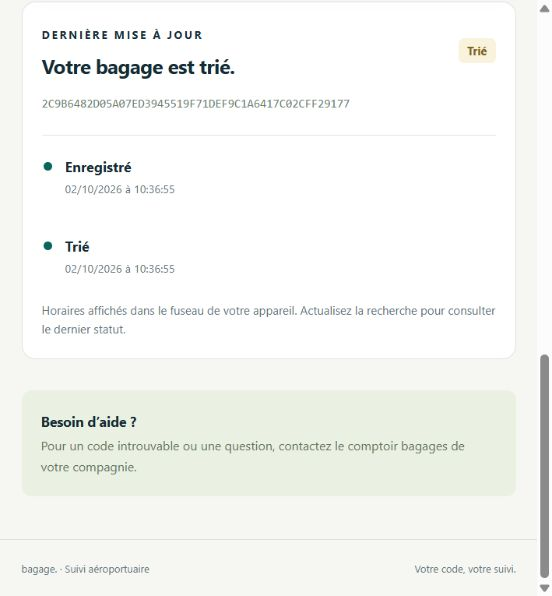
\includegraphics[width=0.62\linewidth,height=0.43\textheight,keepaspectratio]{../docs/captures/recette/01-suivi-internet.jpg}
\caption{Suivi public par URL Internet temporaire}
\label{fig:recette-1}
\end{figure}

\begin{figure}[!htbp]
\centering
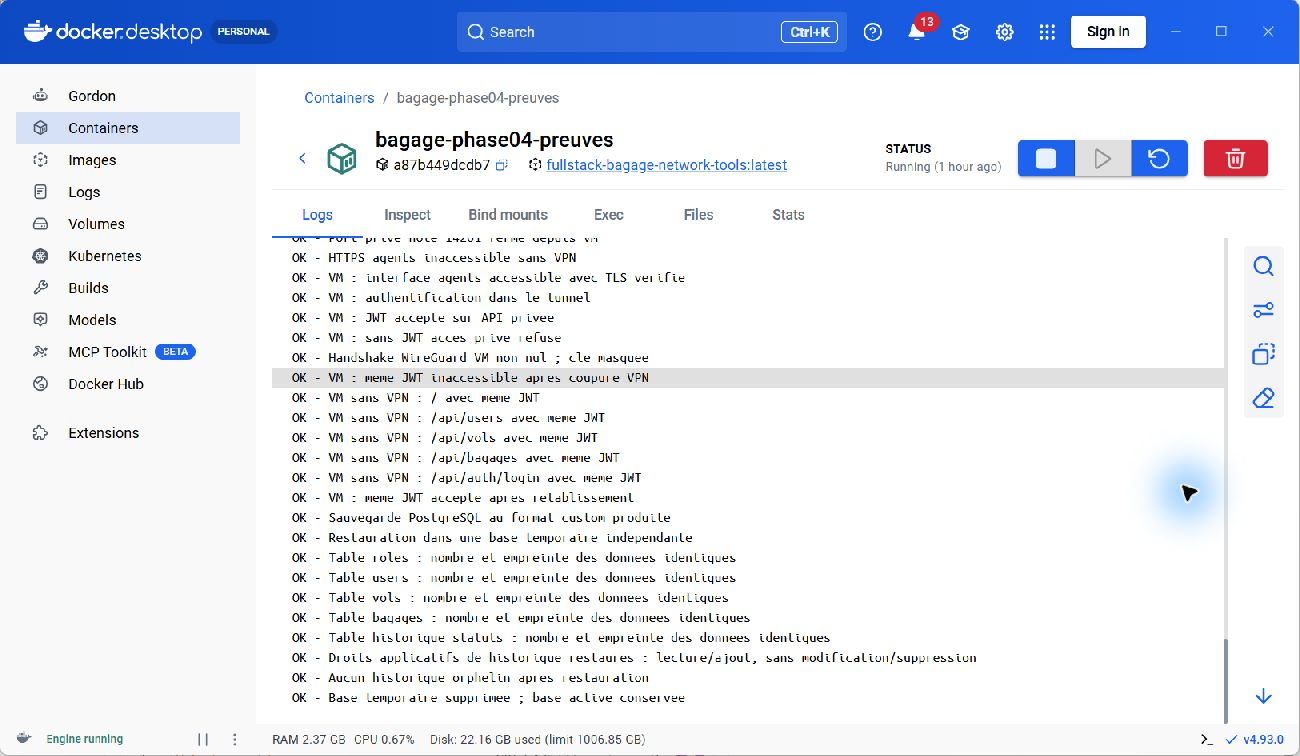
\includegraphics[width=0.96\linewidth,height=0.43\textheight,keepaspectratio,trim=162bp 19.2bp 33bp 117bp,clip]{../docs/captures/recette/02-restauration-postgresql.jpg}
\caption{Restauration logique vérifiée}
\label{fig:recette-2}
\end{figure}

La consultation confirme la continuité du suivi au travers du relais. La restauration logique vérifie l’utilisabilité de la sauvegarde sans remplacer la base active. L’URL temporaire est arrêtée après les essais ; elle ne constitue pas l’hébergement final.

\subsubsection{Valider WireGuard au travers d’un relais UDP public}

Un relais UDP temporaire fournit ensuite un chemin Internet vers WireGuard. La VM réalise le handshake, utilise le JWT, coupe le tunnel et le rétablit. Les contrôles complémentaires vérifient le refus d’un pair inconnu et les restrictions des routes publiques.

\begin{figure}[!htbp]
\centering
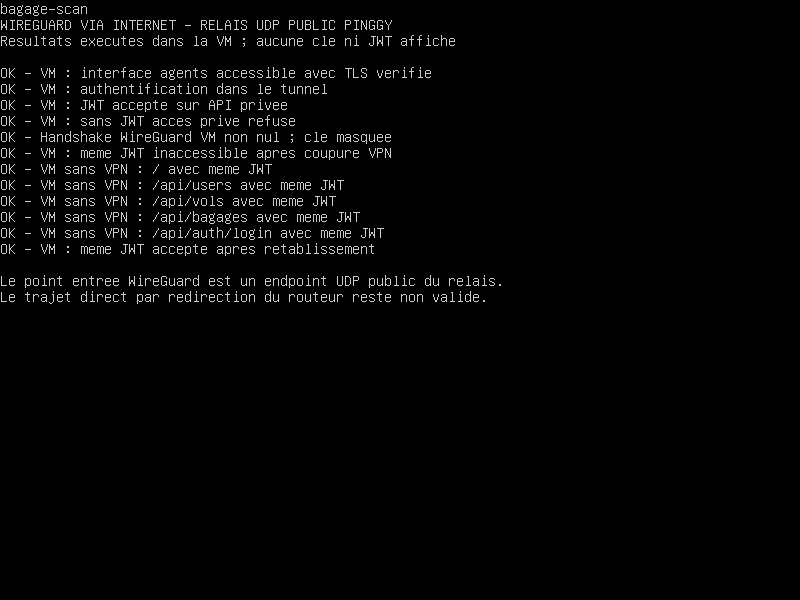
\includegraphics[width=0.96\linewidth,height=0.43\textheight,keepaspectratio,trim=0bp 284bp 287bp 0bp,clip]{../docs/captures/phase-04f/01-wireguard-internet.png}
\caption{WireGuard Internet avec relais public}
\label{fig:phase-04f-1}
\end{figure}

\begin{figure}[!htbp]
\centering
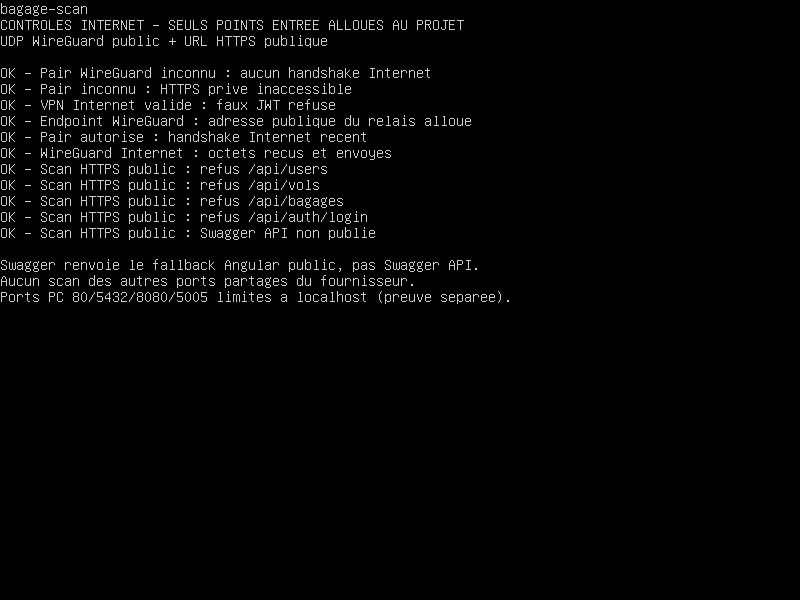
\includegraphics[width=0.96\linewidth,height=0.43\textheight,keepaspectratio,trim=0bp 284bp 279bp 0bp,clip]{../docs/captures/phase-04f/02-controles-internet.png}
\caption{Restrictions et refus d’un pair inconnu}
\label{fig:phase-04f-2}
\end{figure}

Ces observations constituent une première validation Internet du tunnel, dans le périmètre du relais. Les services partagés du fournisseur ne sont pas scannés et le relais est arrêté après utilisation. Pour la soutenance, ce mécanisme temporaire est remplacé par un VPS disposant de son propre point d’entrée.

\FloatBarrier
\subsection{Hébergement OVH : rendre la démonstration indépendante du poste}

\subsubsection{Publier le service passager avec un certificat reconnu}

Le déploiement est transféré vers le VPS Ubuntu 24.04. Le point d’entrée HTTPS public utilise un certificat Let’s Encrypt reconnu et sert l’application Angular. Le parcours de suivi est repris avec un bagage fictif pour vérifier que les réponses proviennent désormais du serveur distant.

\begin{figure}[!htbp]
\centering
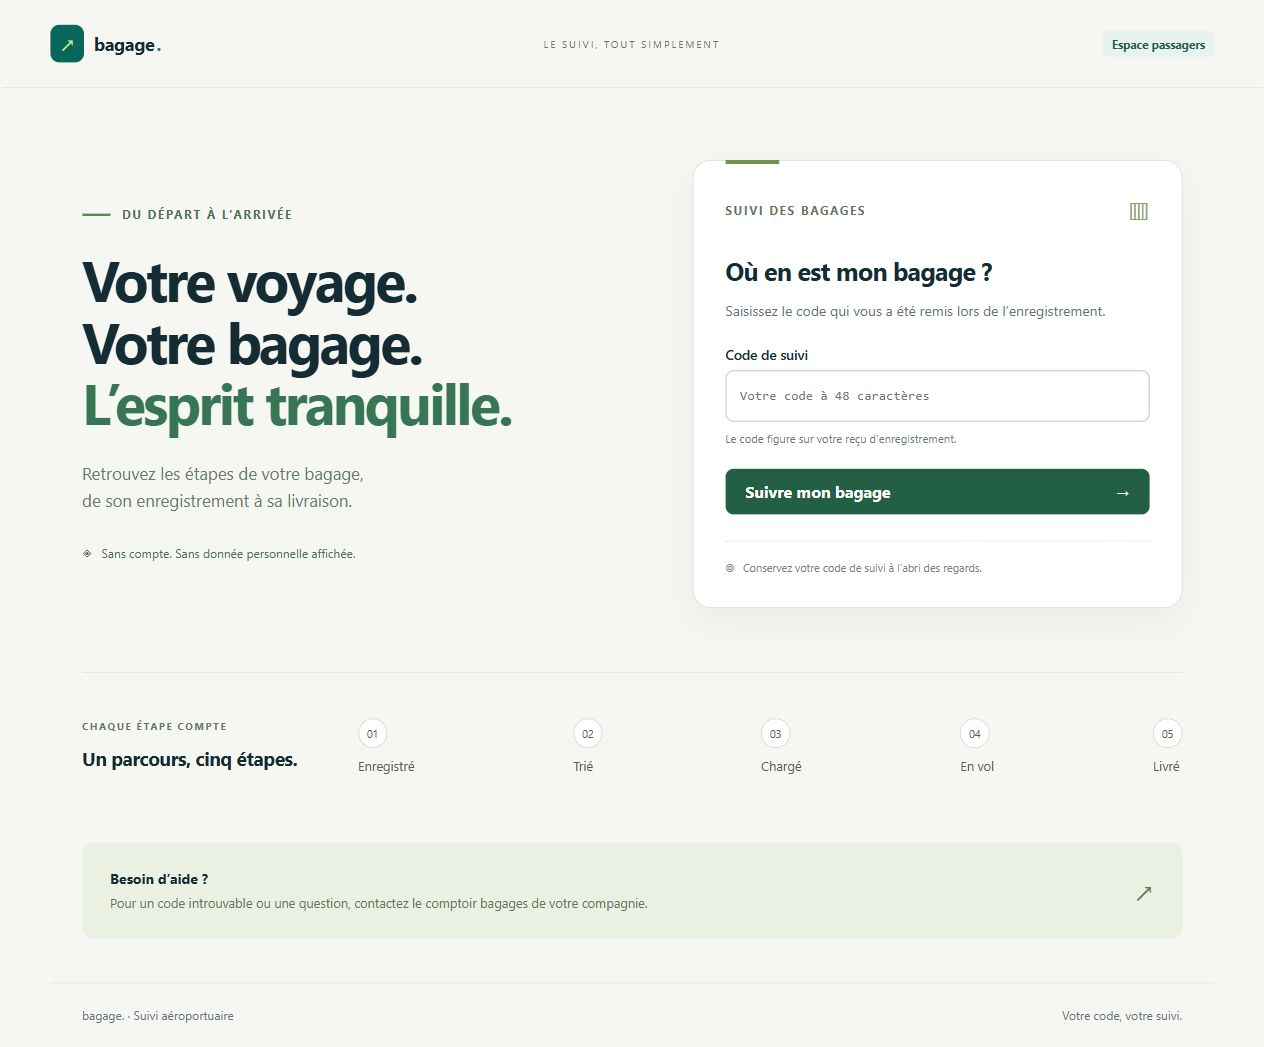
\includegraphics[width=0.96\linewidth,height=0.56\textheight,keepaspectratio]{../docs/captures/phase-05/01-site-public.jpg}
\caption{Application publique hébergée sur OVH}
\label{fig:phase-05-1}
\end{figure}

\begin{figure}[!htbp]
\centering
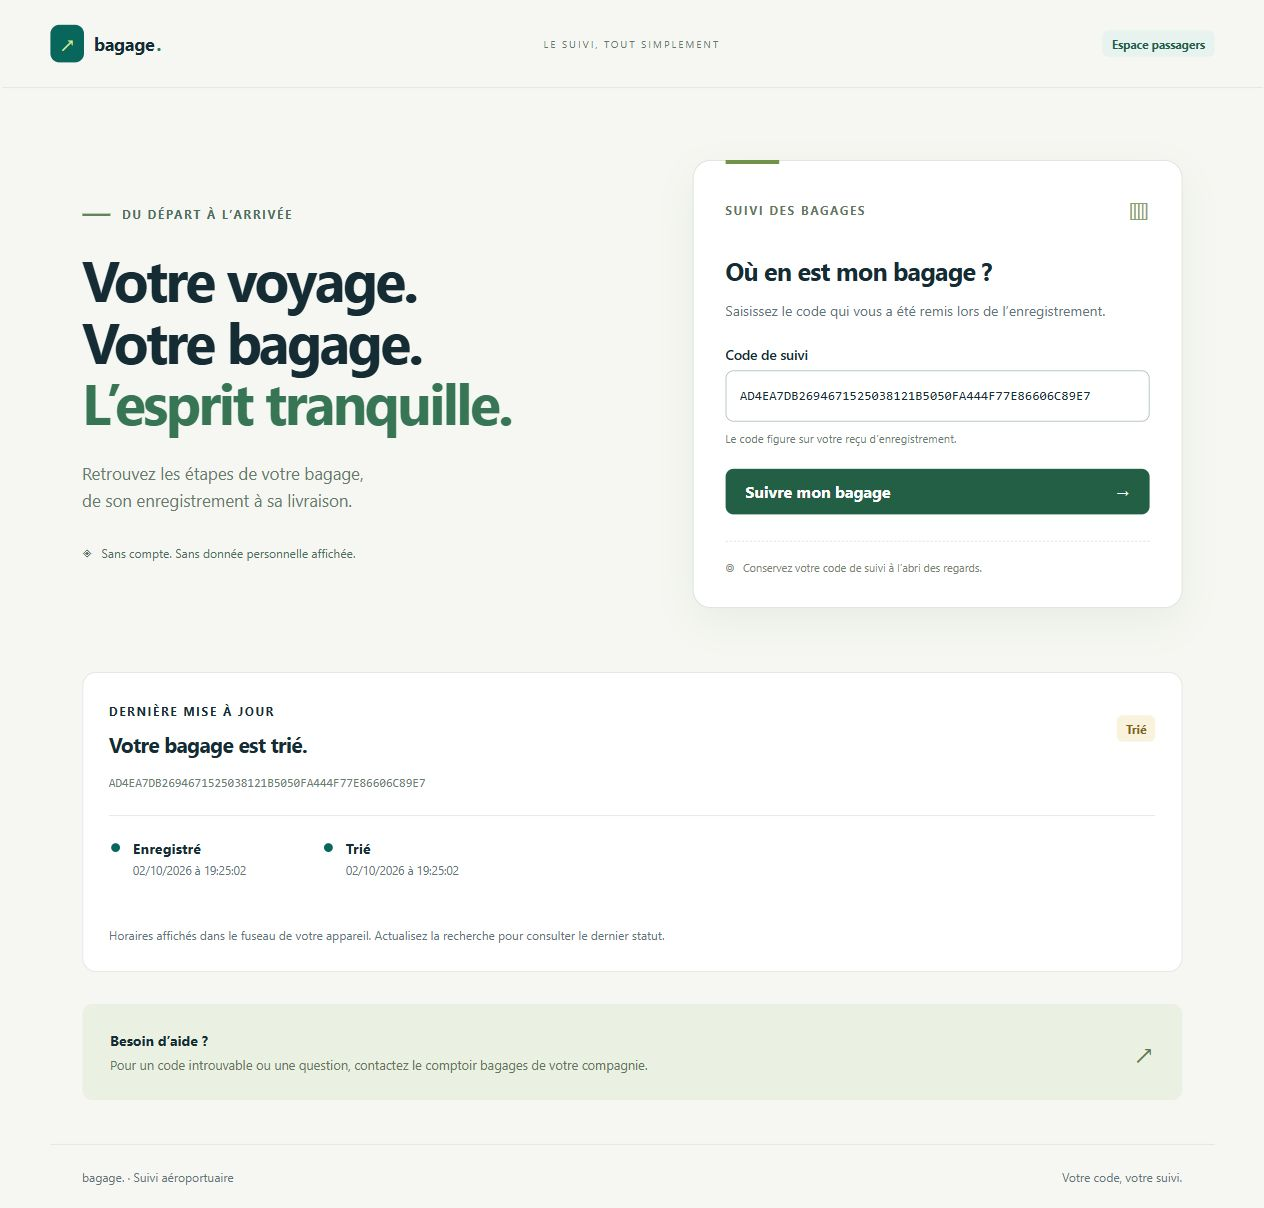
\includegraphics[width=0.62\linewidth,height=0.43\textheight,keepaspectratio]{../docs/captures/phase-05/02-suivi-reel.jpg}
\caption{Suivi du bagage fictif sur OVH}
\label{fig:phase-05-2}
\end{figure}

Le site public est disponible tant que le VPS et son abonnement restent actifs, même lorsque le poste local est éteint. Le statut Trié et les deux événements sont conservés sur OVH ; aucune identité du passager n’est affichée.

\subsubsection{Contrôler la frontière privée depuis Internet}

WireGuard écoute directement sur UDP 52820 du VPS. La VM vérifie l’inaccessibilité des fonctions privées sans VPN et les huit ports TCP sensibles documentés. Sur Windows, le tunnel autorisé permet ensuite de charger l’interface agents en HTTPS avec son certificat privé reconnu.

\begin{figure}[!htbp]
\centering
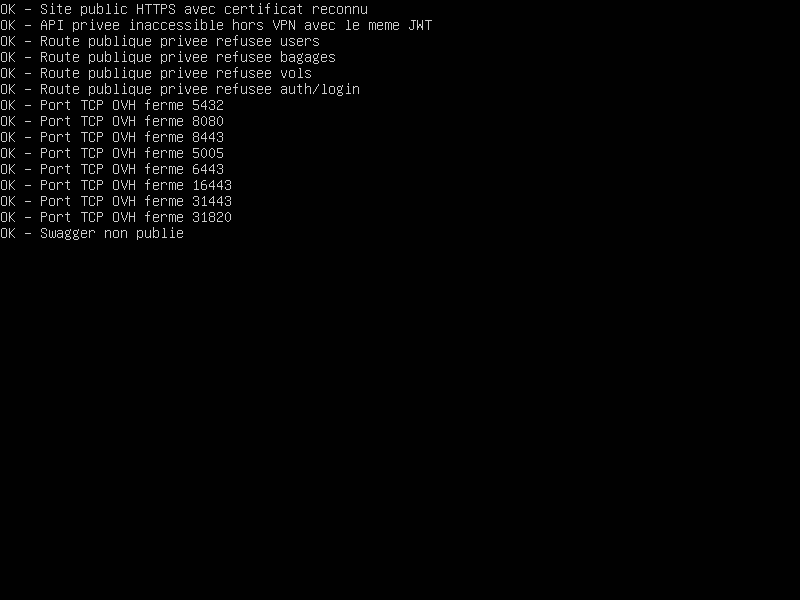
\includegraphics[width=0.96\linewidth,height=0.56\textheight,keepaspectratio,trim=0bp 348bp 356bp 0bp,clip]{../docs/captures/phase-05/03-scan-internet-vm.png}
\caption{Scan Internet du VPS sans VPN}
\label{fig:phase-05-3}
\end{figure}

\begin{figure}[!htbp]
\centering
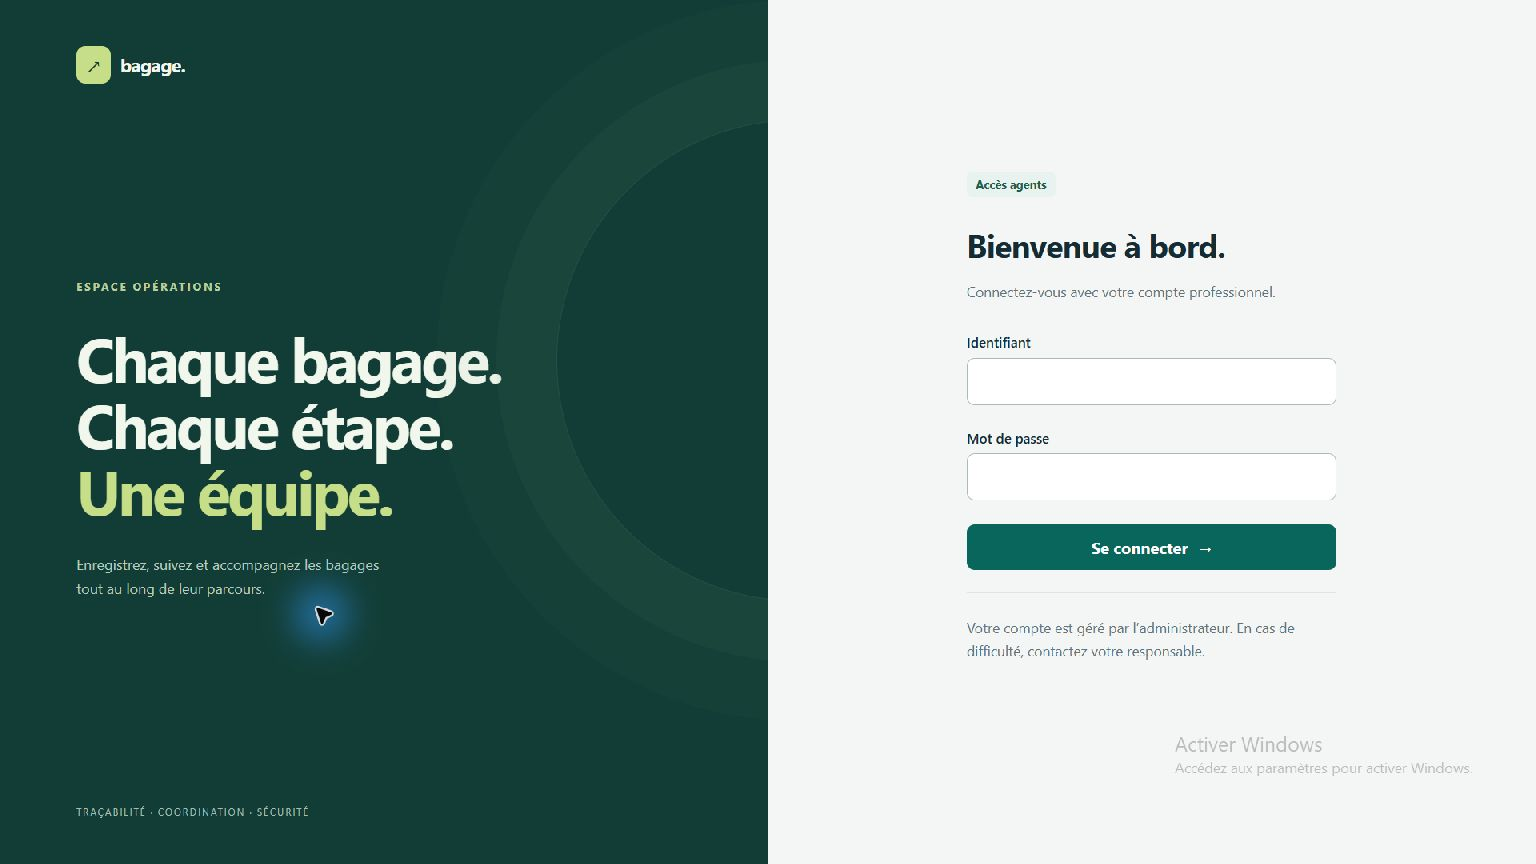
\includegraphics[width=0.96\linewidth,height=0.43\textheight,keepaspectratio]{../docs/captures/phase-05/04-interface-agents-vpn.png}
\caption{Interface agents atteinte par WireGuard OVH}
\label{fig:phase-05-4}
\end{figure}

La page de connexion montre le chargement réel de l’interface privée, sans prétendre représenter une session métier déjà ouverte. Les scénarios API complètent cette observation : refus sans jeton, refus d’un pair inconnu, coupure et rétablissement avec le même JWT. Les vérifications IPv4 et IPv6 portent sur les routes et ports documentés, sans revendiquer un scan exhaustif.

\subsubsection{Assurer la maintenance et vérifier la reprise}

L’administration SSH utilise une clé ; les mots de passe SSH sont désactivés après validation de cet accès. Le renouvellement du certificat public est simulé et son hook met à jour le secret TLS. PostgreSQL~\cite{postgresql} fournit \texttt{pg\_dump} pour les sauvegardes logiques : un dump quotidien est planifié à 02:15 UTC et les sept dernières sauvegardes réussies sont conservées.

Une copie manuelle hors VPS possède la même empreinte que le dump serveur. La restauration est vérifiée dans une base distincte. Enfin, un redémarrage réel du VPS remet les quatre pods applicatifs en état prêt et conserve les trois bagages de démonstration. Ces résultats vérifient la reprise après redémarrage, pas la haute disponibilité ni la perte complète du nœud.

\FloatBarrier
\subsection{Bilan de validation et correspondance avec le cahier des charges}

La validation reprend les critères du tableau~\ref{tab:acceptation} : chaque propriété est reliée à une condition de réussite et à une preuve. Elle associe appels HTTP, parcours métier, accès réseau et observations dans les interfaces. Les rejeux ne sont pas comptés deux fois. Le bilan OVH rassemble les contrôles suivants, exécutés après le déploiement distant.

\begin{table}[htbp]\centering\caption{Contrôles OVH réussis enregistrés le 2 octobre 2026}
\begin{tabular}{lr}\toprule
\textbf{Groupe} & \textbf{Nombre}\\\midrule
Recette métier & 49\\
Internet depuis Docker & 39\\
Internet depuis VMware & 32\\
Infrastructure et durcissement & 26\\
Restauration & 10\\
Windows natif & 5\\
IPv6 & 13\\\midrule
\textbf{Total OVH} & \textbf{174}\\\bottomrule
\end{tabular}\end{table}
Les 281 contrôles et observations antérieurs portent le bilan à 455. Ce nombre ne mesure pas la couverture des tests et ne constitue pas une certification de sécurité.


\begin{longtable}{p{4.2cm}p{6.8cm}p{2.5cm}}
\caption{Traçabilité des exigences et de leur validation}\\\toprule
\textbf{Exigence} & \textbf{Réalisation et preuve} & \textbf{Périmètre}\\\midrule\endfirsthead
\toprule\textbf{Exigence} & \textbf{Réalisation et preuve} & \textbf{Périmètre}\\\midrule\endhead
Suivi public sans identité & Formulaire Angular, route de suivi dédiée ; captures phases 1, 2 et 5. & Local et OVH\\
Enregistrement et cycle métier & Parcours des rôles, transitions normales, perte et correction motivée ; recette métier. & Application\\
Authentification et rôles & JWT vérifié, refus sans jeton et avec rôle insuffisant ; comptes séparés. & API\\
Traçabilité obligatoire & Événements atomiques, horodatages, agent et motif ; historique et recette. & Base et API\\
Accès privé par VPN & Coupure/rétablissement avec le même JWT, pair inconnu refusé ; phases 3 à 5. & Réseau\\
Absence d'exposition PostgreSQL & Service privé et scans des ports connus depuis les clients de test. & Ports testés\\
Déploiement Kubernetes & Deployments, StatefulSet, PVC, Jobs et NetworkPolicy ; sorties kubectl. & Un seul nœud\\
Sauvegarde et restauration & Dump quotidien sur OVH, restauration logique séparée et copie manuelle hors VPS. & Démonstration\\
Rapport et preuves & Guides, résultats expurgés, 37 captures présentées et leurs empreintes. & Livrables\\\bottomrule
\end{longtable}

\FloatBarrier
\subsection{Analyse des résultats et portée des tests}
Les résultats sont interprétés en fonction de la propriété réellement vérifiée. Le refus attendu d'une opération interdite est un succès du contrôle de sécurité. Les tests fonctionnels et les tests réseau répondent à des questions différentes et se complètent.
{\setstretch{1.15}
\begin{longtable}{p{3.1cm}p{5.7cm}p{4.6cm}}
\caption{Interprétation des validations et limites de leurs conclusions}\\\toprule
\textbf{Expérience} & \textbf{Conclusion étayée} & \textbf{Limite}\\\midrule\endfirsthead
\toprule\textbf{Expérience} & \textbf{Conclusion étayée} & \textbf{Limite}\\\midrule\endhead
Sans JWT ou rôle insuffisant & L'API refuse les opérations non autorisées dans les scénarios testés. & Ne démontre pas à elle seule la fermeture d'un service réseau.\\
Même JWT avec coupure VPN & L'accès privé dépend du tunnel, en plus du jeton valide. & Porte sur les routes et clients testés.\\
Suivi public et routes privées & Le passager obtient un suivi limité ; le proxy ne relaie pas les fonctions internes testées. & Le code de suivi doit rester confidentiel.\\
Pair WireGuard inconnu & Le client non configuré ne crée pas le chemin privé attendu. & Ne constitue pas un audit cryptographique du protocole.\\
Ports sensibles IPv4/IPv6 & Les sondes extérieures ne rejoignent pas les ports privés documentés. & Scan limité, sans couverture de tous les ports.\\
Remplacement du pod DB & Les données survivent à la recréation du pod grâce au volume. & Pas de preuve de reprise après perte du disque.\\
Dump et restauration & La copie logique restaure les tables, leurs données et les droits contrôlés. & Restauration sur le même serveur ; copie hors VPS manuelle.\\
Redémarrage OVH & Les services redémarrent et les bagages contrôlés sont conservés. & Pas de haute disponibilité ni test de charge.\\\bottomrule
\end{longtable}
}
Le nombre de contrôles traduit l'étendue des expériences consignées, et non un pourcentage de couverture du code. Les captures complètent les résultats textuels : elles rendent visible l'usage ou l'exécution, sans remplacer le détail des assertions. La conclusion retenue est celle d'un démonstrateur fonctionnel et sécurisé dans le périmètre présenté.
\FloatBarrier
\subsection{Apports du travail et compétences mobilisées}
Le travail réalisé associe trois contributions : la traduction des responsabilités métier en opérations contrôlées, la construction d'une frontière réseau distincte de l'authentification, et la préparation d'un déploiement accompagné de preuves reproductibles. La valeur de la réalisation réside dans leur articulation : le même parcours est conservé lorsque l'environnement évolue du poste local vers Docker, Kubernetes puis OVH.

\subsubsection{Décisions de conception et enseignements}
La séparation des applications et des proxys évite de confondre un menu masqué avec une route protégée. Le compte administrateur dédié limite également le mélange entre gestion des utilisateurs et opérations sur les bagages. Ces décisions traduisent le moindre privilège en comportements que la recette peut observer.

La distinction entre un client Docker, une VM et un client passant réellement par Internet constitue un autre enseignement. Une VM apporte un environnement différent, mais sa présence sur le même poste ne prouve pas à elle seule un trajet extérieur. Le VPS et les essais depuis les clients documentés permettent de préciser le périmètre réel des résultats, sans généraliser une preuve locale.

Le passage à Kubernetes impose enfin de séparer le cycle de vie du conteneur de celui des données. Le volume protège les données lors du remplacement du pod ; la sauvegarde répond à un autre besoin. La restauration dans une base distincte apporte une preuve supplémentaire, sans démontrer une reprise après perte totale de l'hôte.

\subsubsection{Livrables et autonomie de reproduction}
Les sources, migrations, manifestes, scripts et guides constituent les livrables techniques. Les commandes documentées et les résultats associés permettent de reprendre une étape, de localiser la protection testée et de préparer la démonstration. Les captures illustrent les observations ; les assertions conservées dans les comptes rendus apportent les critères de validation. Cette distinction renforce la qualité du dossier au-delà de la seule présentation des interfaces.

Le travail mobilise la modélisation des données, le développement d'une API et d'interfaces, l'administration Linux, la conteneurisation, la segmentation et l'analyse des flux réseau. Il montre aussi l'importance de distinguer une réussite fonctionnelle d'une preuve de sécurité, et une persistance locale d'une stratégie complète de reprise.
\FloatBarrier
\subsection{Limites et perspectives}

La réalisation constitue un démonstrateur mono-nœud. La copie hors VPS reste manuelle, les alertes continues ne sont pas validées et la perte complète du disque n’a pas été simulée. Une exploitation réelle demanderait une stratégie de haute disponibilité, de sauvegarde hors site automatisée, de supervision et de gestion des mises à jour.

\FloatBarrier
\subsection{Conclusion du chapitre}

La progression part d’une chaîne API--base fonctionnelle, la rend utilisable par les différents rôles, puis ajoute les frontières réseau et la persistance. Les clients Windows et VMware élargissent la validation ; le VPS termine la démarche en fournissant un hébergement Internet direct. Chaque série de captures intervient ainsi dans l’explication du résultat qui permet de passer à l’étape suivante.
\FloatBarrier
\fronttitle{Conclusion générale}
Ce projet répond à la problématique de suivi des bagages en associant une application métier à une séparation explicite des accès publics et privés. Le passager consulte un code de suivi sans identité exposée ; les agents interviennent selon leur rôle, au travers du réseau autorisé. L'historique conserve les changements d'état et les corrections motivées.

La démarche a progressé du modèle de données et de l'API vers les interfaces Angular, puis vers WireGuard, Kubernetes et l'hébergement OVH. Les validations montrent le fonctionnement des parcours, le refus des accès interdits, la persistance après remplacement d'un pod et la reprise après redémarrage. La restauration logique complète ces observations. Les résultats restent associés aux clients, routes et expériences documentés.

L'apport du projet est de relier les autorisations applicatives à une frontière réseau vérifiable et de fournir des configurations, scripts et preuves reproductibles. Cette réalisation développe des compétences complémentaires en développement, administration système et sécurité des infrastructures, en cohérence avec la spécialité ARSI.

Les perspectives concernent la haute disponibilité, la sauvegarde hors site automatisée, les alertes de supervision, les tests de charge et une revue de sécurité indépendante. Leur mise en œuvre nécessiterait de nouveaux essais et des ressources adaptées. Le résultat actuel constitue une base de démonstration pour la soutenance ; il n'est pas présenté comme une infrastructure aéroportuaire de production.
\clearpage
\phantomsection\addcontentsline{toc}{section}{Références bibliographiques}
\begin{thebibliography}{99}
\small
\bibitem{jwt} M. Jones, J. Bradley et N. Sakimura, \textit{JSON Web Token (JWT)}, RFC 7519, mai 2015. \url{https://www.rfc-editor.org/rfc/rfc7519}.
\bibitem{wireguard} WireGuard, \textit{Conceptual Overview}, documentation officielle. \url{https://www.wireguard.com/}.
\bibitem{docker} Docker, \textit{What is a container?}, documentation officielle. \url{https://docs.docker.com/get-started/docker-concepts/the-basics/what-is-a-container/}.
\bibitem{kubernetes} Kubernetes, \textit{Network Policies}, documentation officielle. \url{https://kubernetes.io/docs/concepts/services-networking/network-policies/}.
\bibitem{angular} Angular, \textit{What is Angular?}, documentation officielle. \url{https://angular.dev/overview}.
\bibitem{postgresql} PostgreSQL Global Development Group, \textit{PostgreSQL 16 Documentation}, notamment le chapitre 26 sur la sauvegarde et la restauration. \url{https://www.postgresql.org/docs/16/index.html}.
\end{thebibliography}

\end{document}
